\documentclass[a4paper,12pt]{article}
\usepackage[paper=a4paper,left=35mm,right=25mm,top=25mm,bottom=20mm]{geometry}
\usepackage[ngerman]{babel}
\usepackage[utf8]{inputenc}
\usepackage{amsmath}
\usepackage{amssymb}
\usepackage{tikz}
\usepackage{pgfplots}
\usepackage{enumitem}
\usepackage{cite}
\usepackage[square,sort,comma,numbers]{natbib}
\usepackage{graphicx}
\usepackage{float}

\linespread{1.5}

\addto\captionsngerman{
  \renewcommand{\contentsname}
    {INHALTSVERZEICHNIS}
}

\newcommand{\code}{\texttt}

\begin{document}
\parindent0cm
\setlength{\abovedisplayskip}{-1cm}
\setlength{\belowdisplayskip}{0.75cm}

%===================================================================================
%---------------------------- TITELSEITE -------------------------------------------
%===================================================================================

\thispagestyle{empty}

\begin{center}

\begin{large} 
GYMNASIUM OTTOBRUNN	\\
\vspace{1cm}
Oberstufenjahrgang 2017/19\\
\vspace{1cm}
Seminarfach Softwareentwicklung\\
\vspace{2cm}
Seminararbeit\\
\end{large}


\vspace{1cm}


{\Huge\bfseries 
36. Bundeswettbewerb Informatik\par
Runde 2\par
Aufgabe 1 und 3\par 
}


\vspace{2cm}


\begin{large}
\begin{tabular}{rl}
Verfasser:& Jonas Fritsch \\
Seminarleiter: & StD Peter Brichzin \\
Bewertung:  & ......... Punkte  \\
Unterschrift des Seminarleiters: & ...........................................  \\
\end{tabular} 
\end{large}

\end{center}

%===================================================================================
%---------------------------- INHALTSVERZEICHNIS -----------------------------------
%===================================================================================				

\newpage

\thispagestyle{empty}
\tableofcontents	
\thispagestyle{empty}



%===================================================================================
%-------------------------------- EINLEITUNG ---------------------------------------
%===================================================================================

\newpage
\setcounter{page}{4}
\section{EINLEITUNG}



Der aus drei Runden bestehende Bundeswettbewerb Informatik (BwInf) ist einer von vier bundesweiten Informatikwettbewerben. Mit dem 36. BwInf 2017 gab es für die erste Runde mit \textbf{1463} Teilnehmern eine so hohe Teilnahme wie seit 1993 nicht mehr \cite{bwinf_runde1_ergebnis}. Von den ursprünglich 1463 Teilnehmern der ersten Runde haben es \textbf{828} Teilnehmende geschafft, sich für die zweite Runde zu qualifizieren \cite{bwinf_runde2_ergebnis}. Von diesen haben jedoch nur noch \textbf{154} Teilnehmer der zweiten Runde Lösungen für zwei Aufgaben ihrer Wahl eingereicht. Dies lag nicht zuletzt an der stark gestiegenen Komplexität der Aufgaben gegenüber der ersten Runde. Zu der letzten dritten Runde des Bundeswettbewerbs Informatik wurden schlussendlich nur noch \textbf{25} Teilnehmer eingeladen. Das waren im Falle des BwInfs von 2017 nur rund \textbf{1,7\%} der ursprünglichen Teilnehmer.
\\[0.4cm]
Im Folgenden wird eine eingereichte Lösung zu der ersten und dritten Aufgabe der zweiten Runde des 36. Bundeswettbewerbs Informatik erläutert.

%===================================================================================
%-------------------------------- AUFGABE 1 ----------------------------------------
%===================================================================================

\newpage
\section{AUFGABE 1 – „Die Kunst der Fuge“}



\subsection{Aufgabenstellung}
Ilona besitzt einen riesigen Haufen Holzklötzchen: Diese haben alle dieselbe Höhe und Tiefe,
aber verschiedene Längen. \\
Ilona möchte eine Mauer bauen. Jede Reihe der Mauer soll aus $n$ Klötzchen bestehen, die die
Längen 1 bis $n$ haben und lückenlos aneinanderliegen. Die Stellen zwischen den Klötzchen heißen
Fugen. Ilona möchte, dass in der fertigen Mauer niemals zwei Fugen übereinander liegen,
selbst wenn sich mehrere Reihen dazwischen befinden. Außerdem soll ihre Mauer möglichst
hoch sein. \\
Für $n = 4$ gelingt es ihr recht schnell, eine Mauer mit drei Reihen zu bauen:
\begin{figure}[H]
    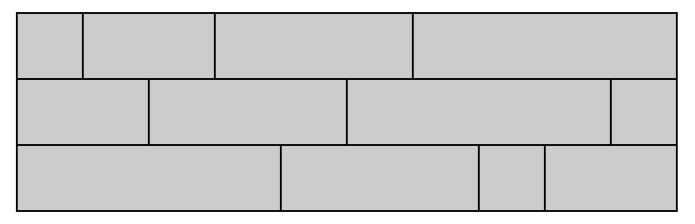
\includegraphics[width=0.7\linewidth]{Bilder/Aufgabe1/Aufgabenstellung_BeispielMauer.png}
\end{figure}
\begin{large}
    \textbf{Aufgabe} \\
\end{large}
Hilf Ilona, indem du ein Programm schreibst, das nach Eingabe von $n$ eine nach ihren Vorgaben
konstruierte, möglichst hohe Mauer ausgibt. Für $n = 10$ sollte dein Programm eine Mauer der
Höhe 6 ausgeben können. Wie hoch werden die Mauern deines Programms für größere $n$?

\subsection{Auslegung der Aufgabe}
Die grundlegende Aufgabe ist es, eine Mauer mit möglichst vielen Reihen, die aus verschieden länglichen Klötzchen bestehen, zu bauen.

Die Variable $n$ ($n \in \mathbb{N}$\textbackslash$\{0\}$) definiert dabei die Längen und auch die Gesamtanzahl der Klötzchen pro Reihe.
Gesamtanzahl heißt, dass bei zum Beispiel $n = 5$ jede Reihe aus 5 einzelnen Klötzchen besteht. 
Jede Reihe setzt sich dann aus einem 1er-, einem 2er-, einem 3er-, einem 4er- und einem 5er-Klötzchen zusammen.
\\[0.4cm]
Der Trick bei der Aufgabe ist nun, dass niemals zwei Fugen \textbf{übereinanderliegen dürfen}.
Eine Fuge ist die Lücke zwischen zwei Klötzchen (siehe Abbildung 1).
\begin{figure}[H]
    \centering
    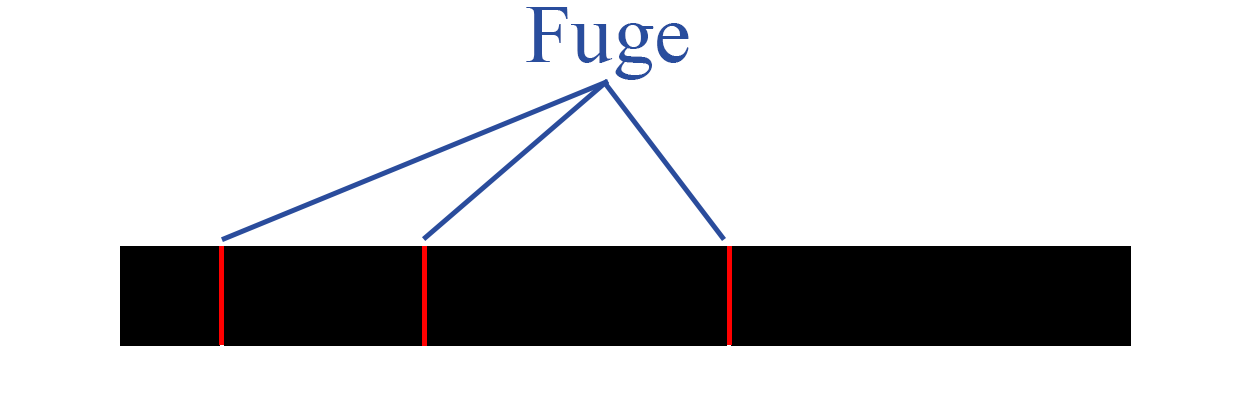
\includegraphics[width=0.8\linewidth]{Bilder/Aufgabe1/Definition_Fuge.png}
    \caption{Darstellung der 3 Fugen einer Reihe mit 4 Klötzchen}
\end{figure}

Als Hilfestellung wurde außerdem erwähnt, dass eine Mauer für $n = 10$ eine maximale Höhe von $6$ hat.

\subsection{Lösungsidee}
\subsubsection{Verstehen des Problems}
Um die Problemstellung der Aufgabe genauer zu verstehen, bietet es sich erstmal an, Mauern für kleinere $n$ auf Papier zu zeichnen.
Beginnt man mit $n = 1$, fällt auf, dass ganz gleich, wie viele Reihen übereinanderliegen, es nie zu einer Fugenüberlappung kommen kann, da eine Reihe mit einem einzelnen Klötzchen keine Fuge besitzt.
Für $n = 1$ kann also theoretisch eine \textbf{unendlich} hohe Mauer gebaut werden.
\\[0.4cm]
Für $n = 2$ ist es auch noch recht einfach, eine Mauer zu bauen. Denn es gibt pro Reihe nur 2 mögliche Reihenfolgen von Klötzchen. Entweder kommt zuerst das 1er- oder das 2er-Klötzchen. 
Eine der zwei möglichen Lösungen ist in Abbildung 2 zu sehen. Es gibt keine Möglichkeit, noch ein Klötzchen in einer neuen dritten Reihe zu platzieren, ohne eine Fuge doppelt zu besetzen.
\begin{figure}[H]
    \centering
    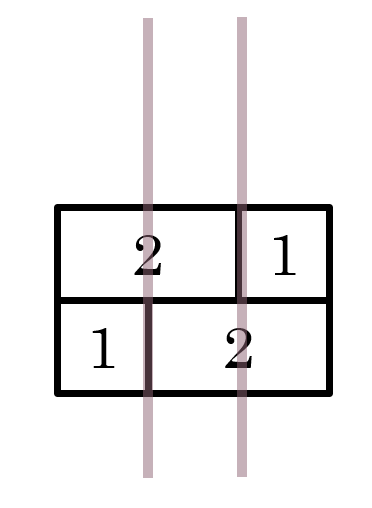
\includegraphics[width=0.25\linewidth]{Bilder/Aufgabe1/Loesung_N2.png}
    \caption{Eine der zwei möglichen Lösungen für $n = 2$. Die vertikalen Striche zeigen an, dass die jeweilige Fuge bereits besetzt ist.}
\end{figure}

Auch für $n = 3$ gibt es eine Mauer mit einer maximalen Höhe von 2 (siehe Abbildung 3). Hier wird es jedoch schon komplexer, da es nun für eine Reihe nicht mehr $2! = 2\times1 = 2$, sondern $3! = 3\times2\times1 = 6$ mögliche Klötzchen-Reihenfolgen gibt.
Außerdem tritt bei $N = 3$ das erste Mal auf, dass eine \textbf{mögliche Fugenstelle nicht besetzt wird.}
\begin{figure}[H]
    \centering
    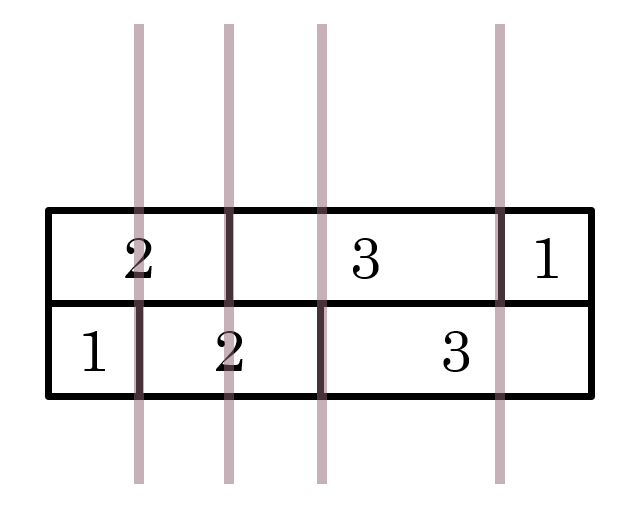
\includegraphics[width=0.4\linewidth]{Bilder/Aufgabe1/Loesung_N3.png}
    \caption{Eine mögliche Lösung für $n = 3$. Zu beachten ist, dass in der Mauer eine \textbf{mögliche} Fugenstelle, dort wo es eine größere Lücke zwischen den zwei letzten besetzten Fugenstellen gibt, \textbf{unbesetzt bleibt.}}
\end{figure}

Geht man noch weiter und bildet eine Mauer für $n = 4$ ($4! = 24$ mögliche Klötzchen Anordnungen pro Reihe), so kann man erstmals eine Mauer der Höhe 3 bilden (siehe Abbildung 4). Hier ist auch wieder jede einzelne Fugenstelle besetzt.
\begin{figure}[H]
    \centering
    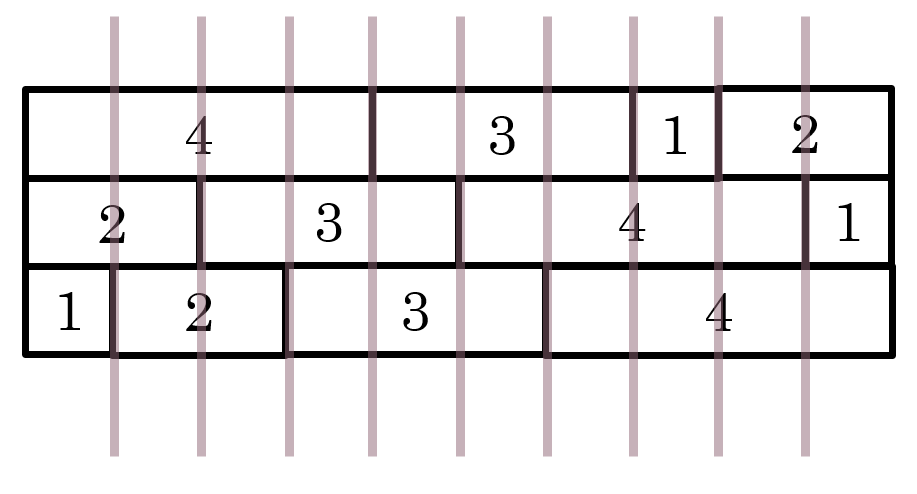
\includegraphics[width=0.6\linewidth]{Bilder/Aufgabe1/Loesung_N4.png}
    \caption{Eine mögliche Lösung für $n = 4$}
\end{figure}

Die Komplexität der Aufgabe steigt mit höheren $n$ stark an. Während man bei $n = 2$ $2!$ Möglichkeiten pro Reihe und 2 Reihen hatte ($2!\times2 = 4$ unterschiedliche Mauern), gibt es bei $n = 4$ bereits $4!\times3 = 72$ verschiedene Mauern.
Allgemein gibt es also für eine Mauer $n!\times h$ Lösungen, wobei $h$ die Anzahl der übereinanderliegenden Reihen ist.
\\[0.4cm]
Es ist logisch, dass zwischen der Anzahl der maximal möglichen Reihen $h$ und der Anzahl der Klötzchen pro Reihe $n$ eine Abhängigkeit existiert.
\\[0.4cm]
Allgemein kann man sagen, dass die \textbf{maximale Mauerhöhe} dann erreicht ist, wenn \textbf{nicht} mehr \textbf{genügend Fugenstellen in der Mauer frei sind}, um eine \textbf{weitere Reihe zu bilden}.

Somit lässt sich die Formel
\begin{center}
\begin{Large}
\[h = \frac{f_{Mauer}}{f_{Reihe}}\]
\end{Large}
\end{center}
ableiten, wobei $f_{Mauer}$ die maximale Anzahl an Fugen in der Mauer und $f_{Reihe}$ die Anzahl der Fugen, die eine Reihe besetzt, beschreibt.
\\[0.4cm]
Um nun auf $f_{Mauer}$ schließen zu können, braucht man nur die Länge der Mauer. Da jede Reihe der Mauer gleich lang ist, ist die Länge der Mauer gleich der Länge einer Reihe. Die Länge einer Reihe definiert sich wiederum durch die Menge und Breite ihrer Klötzchen. Das heißt also, die Länge einer Reihe/der Mauer ist nach der \textbf{Gaußschen Summenformel}
% TODO: Quelle für Gaußsche Summenformel
\begin{center}
\begin{Large}
\[1+2...+n = \sum_{k=1}^n k = \frac{n(n+1)}{2}\]
\end{Large}
\end{center}
Um nun aber von der Länge der Mauer auf $f_{Mauer}$ zu schließen, muss man noch $1$ von der Länge der Mauer abziehen. Dies wird offensichtlich, wenn man zu einer Mauer eine Reihe aus lauter 1er-Klötzchen bildet (siehe Abbildung 5). Jedes 1er-Klötzchen, bis auf das Letzte, besetzt eine Fuge. Da das Ende des letzten Klötzchens nicht als Fuge gilt, wird von der Länge der Reihe noch $1$ abgezogen.
\begin{figure}[H]
    \centering
    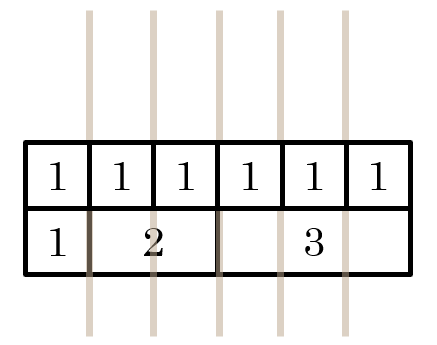
\includegraphics[width=0.4\linewidth]{Bilder/Aufgabe1/Definition_Fugenstellen_Mauer.png}
    \caption{Eine Mauer der Länge 6 besitzt 5 mögliche Fugenstellen.}
\end{figure}

Ähnlich lässt sich auch $f_{Reihe}$ berechnen. Um wissen zu wollen, wie viele freie Fugen eine Reihe mit $n$ Klötzchen besetzen wird, zieht man einfach wieder 1 von der Anzahl der Klötzchen pro Reihe ($n$) ab (siehe Abbildung 6).
\begin{figure}[H]
    \centering
    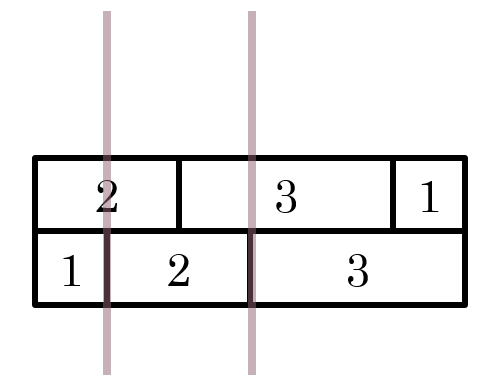
\includegraphics[width=0.4\linewidth]{Bilder/Aufgabe1/Definition_Fugenstellen_Reihe.png}
    \caption{Eine Reihe bei $n = 3$ besetzt $n-1 = 2$ freie Fugen}
\end{figure}

Daraus ergibt sich die fertige Formel für die Anzahl der Reihen $h$ in einer maximal hohen Mauer in Abhängigkeit von $n$.
\begin{center}
\begin{Large}
\[h = \frac{\frac{n\times(n+1)}{2}-1}{n-1} = \frac{n}{2}+1\]
\end{Large}
\end{center}

Der Graph der daraus folgenden Funktion $h(n) = \frac{n}{2}+1$ verläuft dabei linear (siehe Abbildung 7).
\begin{figure}[H]
    \centering
    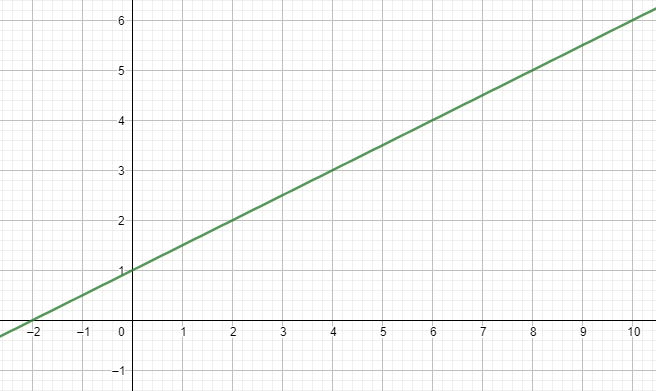
\includegraphics[width=0.95\linewidth]{Bilder/Aufgabe1/Graph_01.png}
    \caption{Graph der linearen Funktion $h(n) = \frac{n}{2}+1$}
\end{figure}
Setzt man nun für $n = 10$ ein, ergibt sich der Funktionswert $6$, der mit der in der Aufgabenstellung angegebenen Höhe für eine Mauer von $n = 10$ übereinstimmt.
Testet man allerdings die maximale Mauerhöhe für zum Beispiel $n = 3$, so ergibt sich als Wert $2,5$. Dies macht allerdings keinen Sinn, da die fertige Mauer nur aus vollen Reihen bestehen muss und keine halbfertige Mauer besitzen kann.
\\[0.4cm]
Jedes ungerade $n$ zieht einen nicht-ganzzahligen Funktionswert $h$ nach sich. Der Zusammenhang ist dabei, dass wie beim vorherigen Beispiel $n = 3$ (siehe Abbildung 3) eine Fuge unbesetzt bleibt. Diese Fuge kann zwar mit einem weiteren Klötzchen besetzt werden, die Reihe könnte aber nicht mehr vollständig gebaut werden.
Da die Mauerhöhe also eine natürliche Zahl sein muss, wird der Funktionsterm noch mit Abrundungsklammern umgeben:
\begin{center}
\begin{Large}
\[h(n) = \lfloor\frac{n}{2}+1\rfloor\]
\end{Large}
\end{center}
Der daraus resultierende Graph ist in Abbildung 8 zu sehen.
\begin{figure}[H]
    \centering
    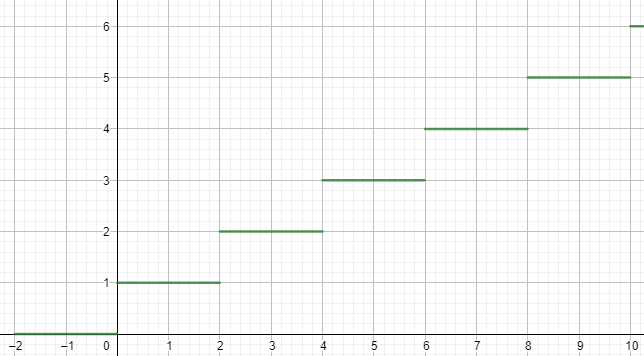
\includegraphics[width=0.95\linewidth]{Bilder/Aufgabe1/Graph_02.png}
    \caption{Graph der Funktion $h(n) = \lfloor\frac{n}{2}+1\rfloor$}
\end{figure}
Somit gibt die Funktion $h(n)$ mit der Definitionsmenge $\mathbb{D}_{h} = \mathbb{N}$\textbackslash$\{0;1\}$ und der Wertemenge $\mathbb{W}_{h} = \mathbb{N}$\textbackslash$\{0\}$ die jeweilige maximale Mauerhöhe ($h$) in Abhängigkeit von $n$ an. Wobei in der Definitionsmenge auch $1$ ausgeschlossen ist, weil für $n = 1$ aus logischer Sicht eine unendlich hohe Mauer und nicht nur eine Mauer der Höhe 1 gebildet werden kann.
\\[0.4cm]
Die naivste Lösung für die Aufgabe bestünde darin, per Brute-Force so viele Mauer-Permutationen durchzugehen, bis man eine fertige Mauer der maximalen Höhe ohne Fugenüberlappung erreicht hat.
\\[0.4cm]
Für die in der Aufgabenstellung festgelegte Mindestanforderung $n = 10$, gäbe es bereits
\begin{center}
\begin{Large}
\[f(10) = 10!^6\approx2,28\mathrm{e}{+39}\]
\end{Large}
\end{center}
\textbf{unterschiedliche Mauerkombinationen} bei der maximalen Mauerhöhe von 6.
Der Graph der allgemeinen Formel
\begin{center}
\begin{Large}
\[f(n) = n!^{\lfloor\frac{n}{2}+1\rfloor}\]
\end{Large}
\end{center}
ist in Abbildung 9 zu sehen.
\begin{figure}[H]
    \centering
    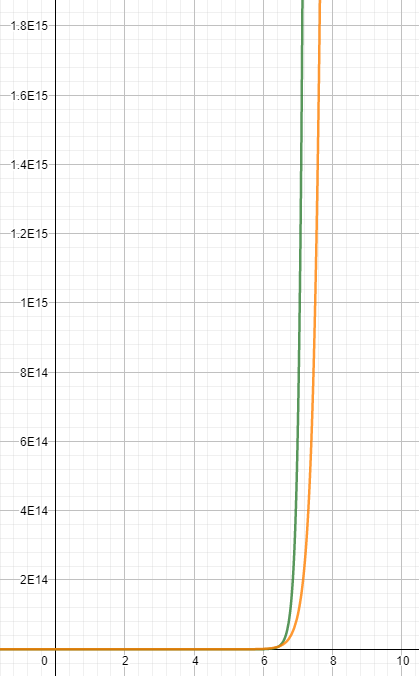
\includegraphics[width=0.7\linewidth]{Bilder/Aufgabe1/Graph_03.png}
    \caption{Der grüne Graph zeigt die extreme Steigung der Funktion 
        $f(n) = n!^{\lfloor\frac{n}{2}+1\rfloor}$. Zum Vergleich der orange farbige Graph der Funktion $g(x) = 100^{x}$.}
\end{figure}
Die Anzahl der verschiedenen möglichen Mauern für $n$ steigt somit mehr als 
\textbf{exponentiell}.
\\[0.4cm]
Nun ist hierbei allerdings zu beachten, dass es durchaus mehrere mögliche unterschiedliche Lösungen geben kann. Unter anderem werden bei der Gesamtmenge unterschiedlicher Mauern auch Mauern unterschieden, die die gleichen Reihen in unterschiedlicher Reihenfolge besitzen (siehe Abbildung 10). Dies führt zu einer Vielzahl möglicher Lösungen.
\begin{figure}[H]
    \centering
    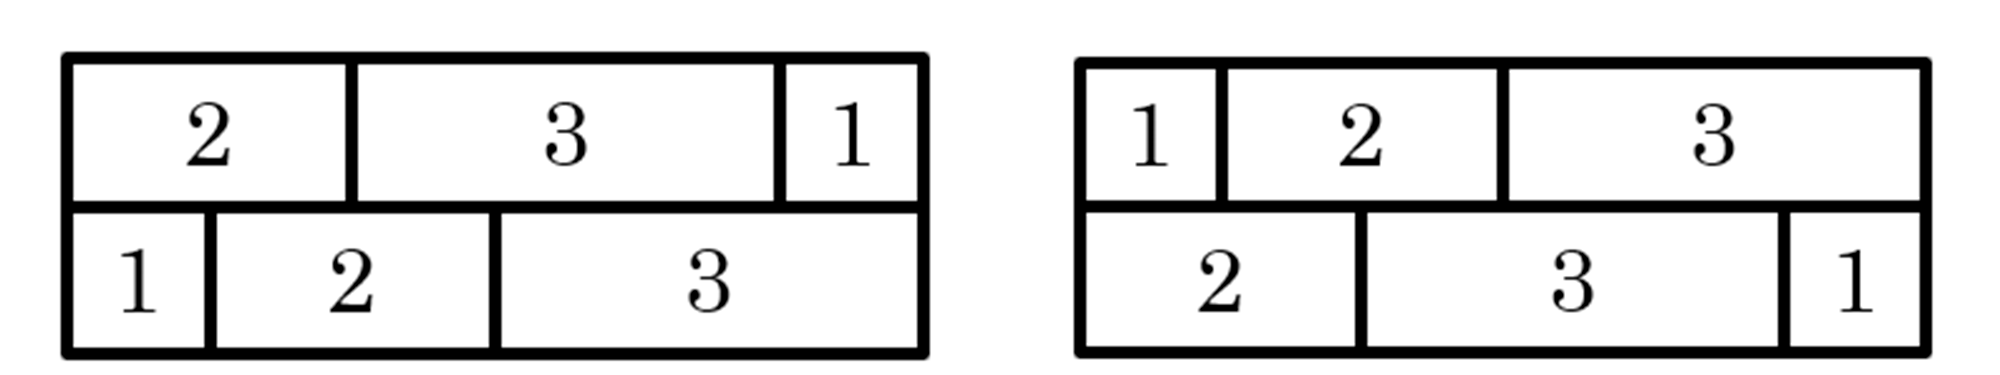
\includegraphics[width=0.9\linewidth]{Bilder/Aufgabe1/Mauervarianten_N3.png}
    \caption{Obwohl beide Mauern aus denselben zwei Reihen bestehen, werden sie als unterschiedliche Mauern angesehen.}
\end{figure}
Weiterhin ist zu beachten, dass es für Mauern mit ungeraden $n$ mehr unterschiedliche Lösungen gibt als für die wieder darauffolgende Mauer mit geraden $n$.

Dies liegt eben daran, dass bei ungeraden $n$ immer mindestens eine Fugenstelle frei bleibt, was wiederum zu mehr richtigen Mauervariationen führt.
\\[0.4cm]
Trotzdem würde das Finden einer Lösung für $n = 10$, selbst wenn ein Computer nur \textbf{1 Millisekunde} für die Permutation einer \textbf{gesamten Mauer} benötigen würde, die maximal erwartete Algorithmuslaufzeit einer BwInf-Lösung bei Weitem überschreiten.
\\[0.4cm]
Damit ist eine naive Brute-Force Methode als Lösung ausgeschlossen und es muss nach einem effizienteren Algorithmus gesucht werden.

\subsubsection{Der Algorithmus}
Grundlegend gibt es zwei unterschiedliche Wege, eine Mauer wie in der Aufgabenstellung zu bauen.
\\[0.4cm]
Der offensichtlichere ist die Bauart \textbf{„Von unten nach oben“}. Bei dieser Bauart setzt man zuerst die Klötzchen zu einer Reihe zusammen. Hat man eine Reihe fertig, beginnt man mit der zweiten Reihe und so weiter (siehe Abbildung 11). Man setzt Reihe auf Reihe (von unten nach oben), bis man die Maximalhöhe erreicht hat.
\begin{figure}[H]
    \centering
    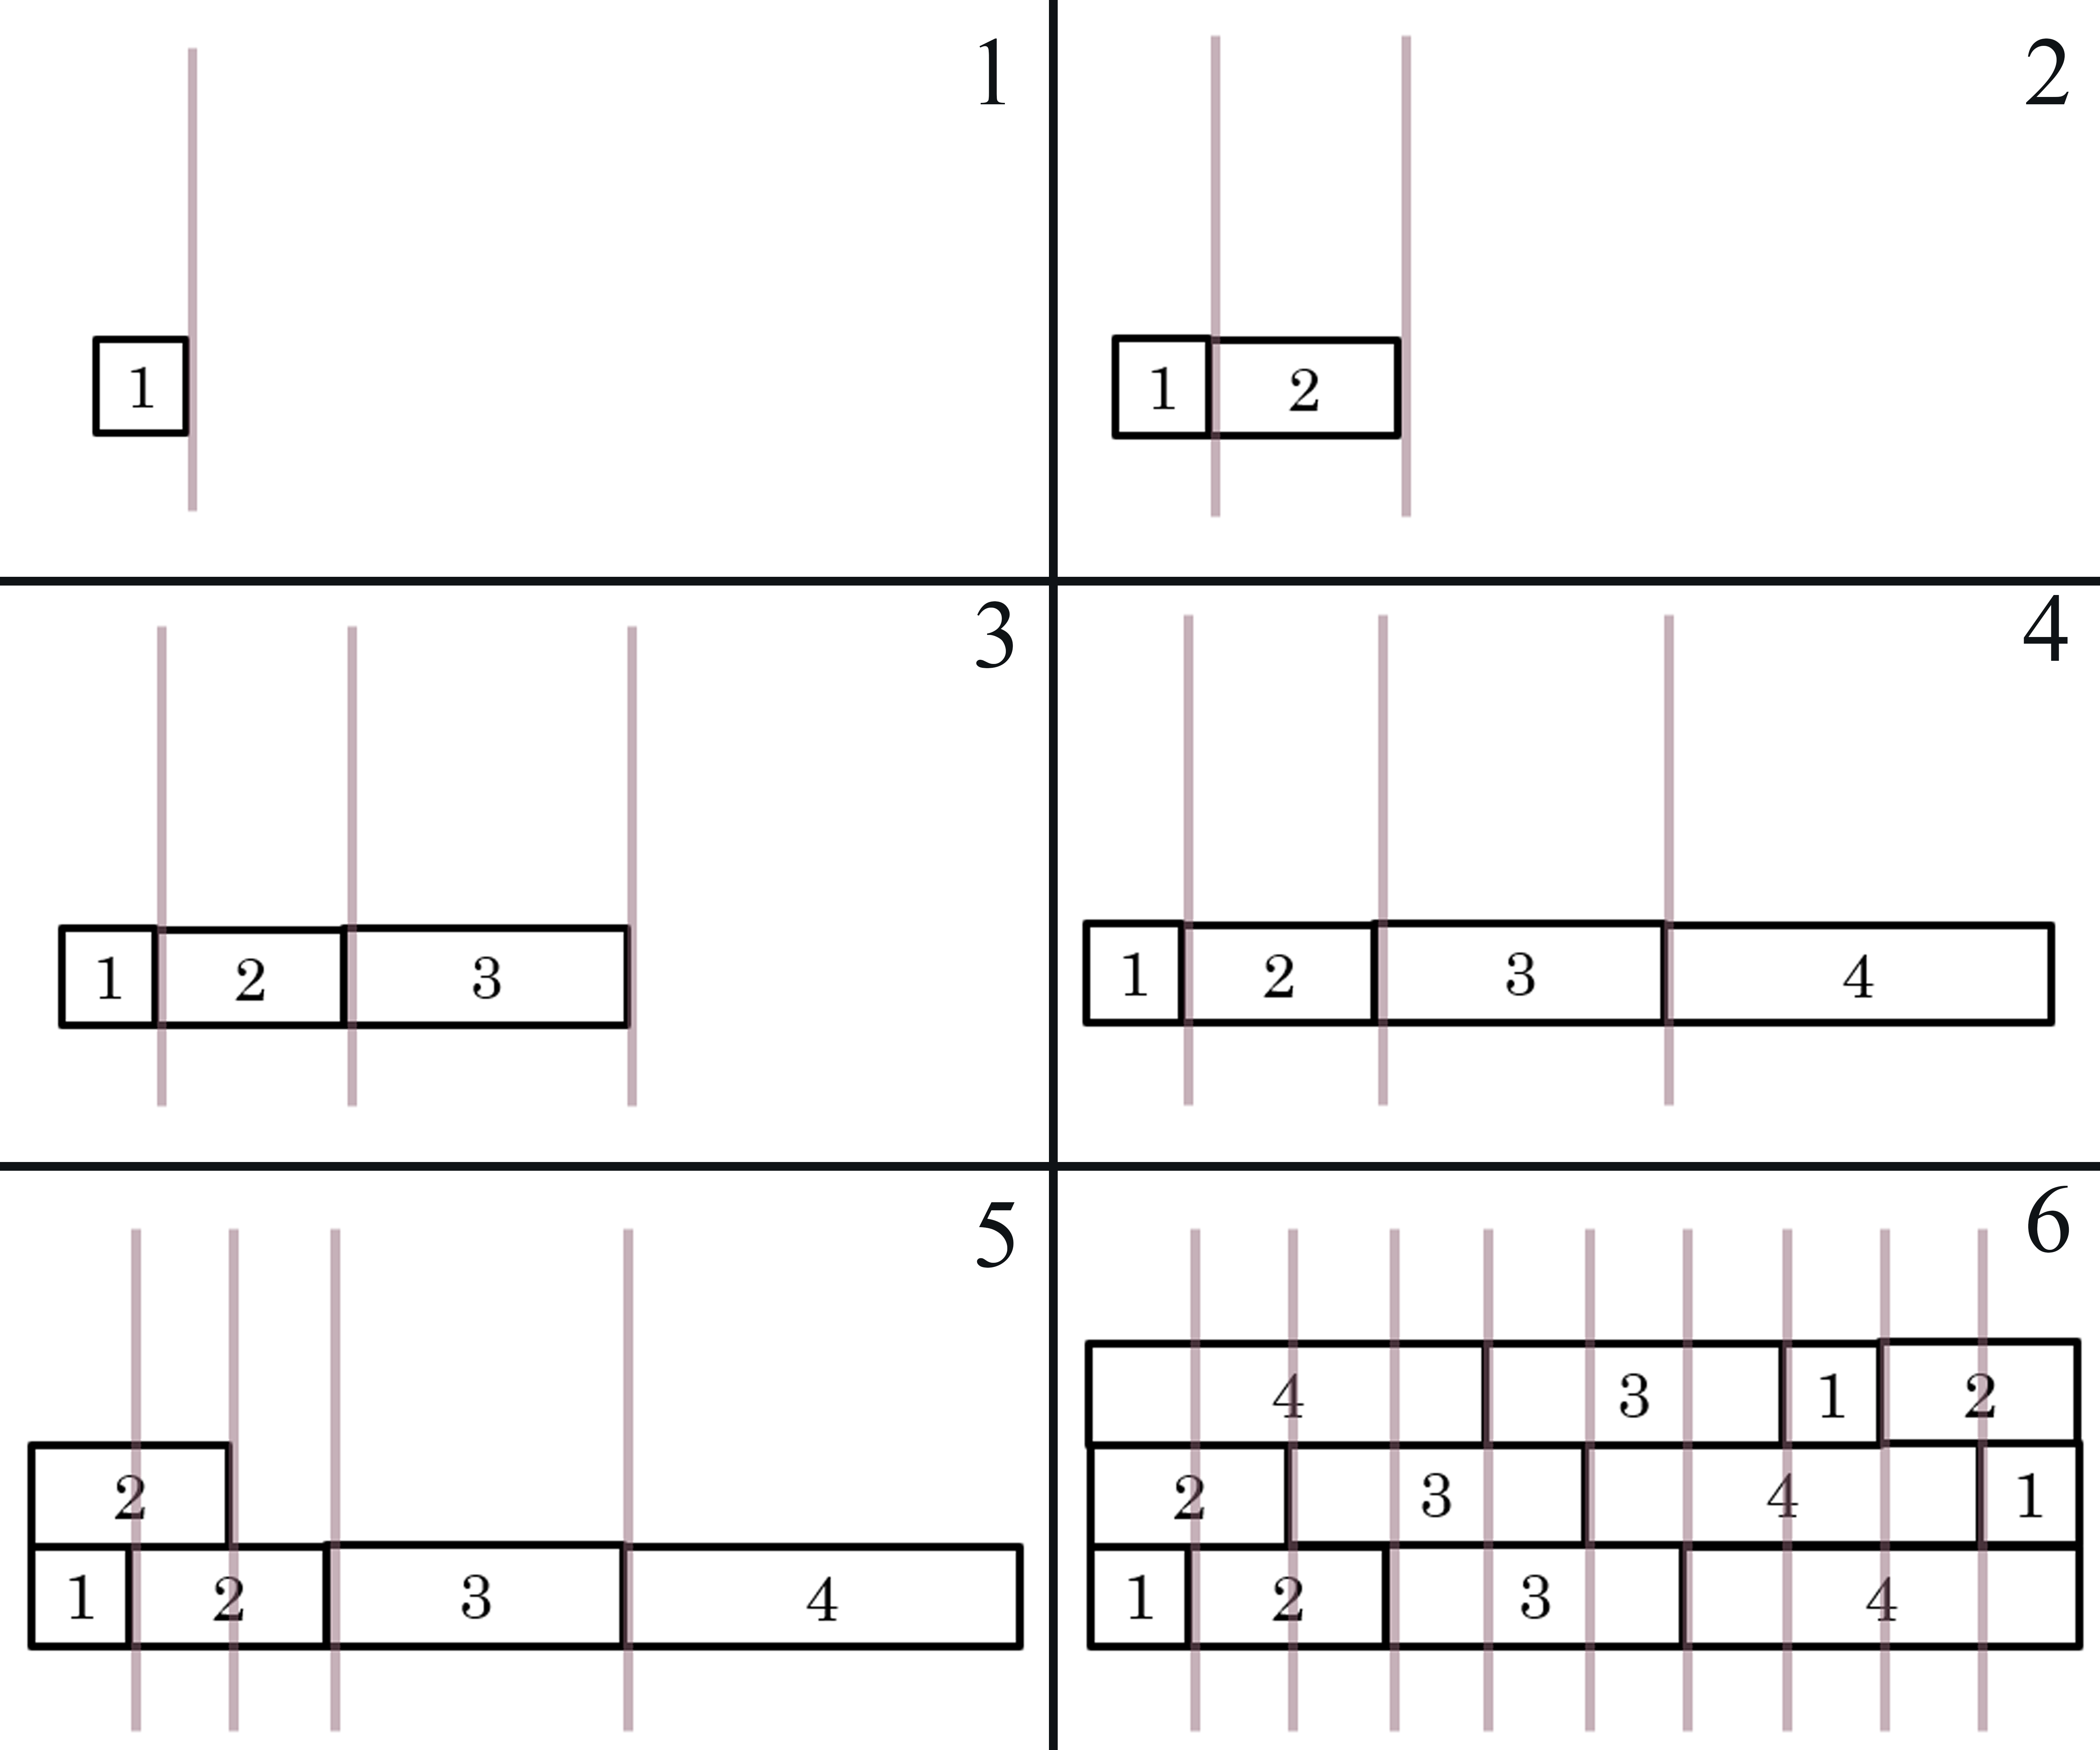
\includegraphics[width=1\linewidth]{Bilder/Aufgabe1/Definition_Mauerbauart_01.png}
    \caption{Der Bau einer Mauer nach der \textbf{„Von unten nach oben“}-Methode. Es wird Reihe nach Reihe gebaut (1-5), bis die maximale Höhe erreicht wurde (6).}
\end{figure}

Eine andere Möglichkeit ist, wenn man die Anzahl der Reihen ($h$) für eine Mauer der maximalen Höhe bereits weiß, die Mauer \textbf{„von links nach rechts“} aufzubauen.
Man kann die Aufgabe auch so formulieren, dass das \textbf{Ziel ist, möglichst alle Fugenpositionen in der Mauer zu füllen}. Nun bietet es sich an, anstatt wie bei \textbf{„von unten nach oben“} immer ein Klötzchen zu setzen und \textbf{dann} zu schauen, ob die jeweilige Fugenposition noch frei ist, von den \textbf{Fugenpositionen auszugehen} und diese jeweils zu versuchen, \textbf{mit einem Klötzchen zu füllen} (siehe Abbildung 12).
\begin{figure}[H]
    \centering
    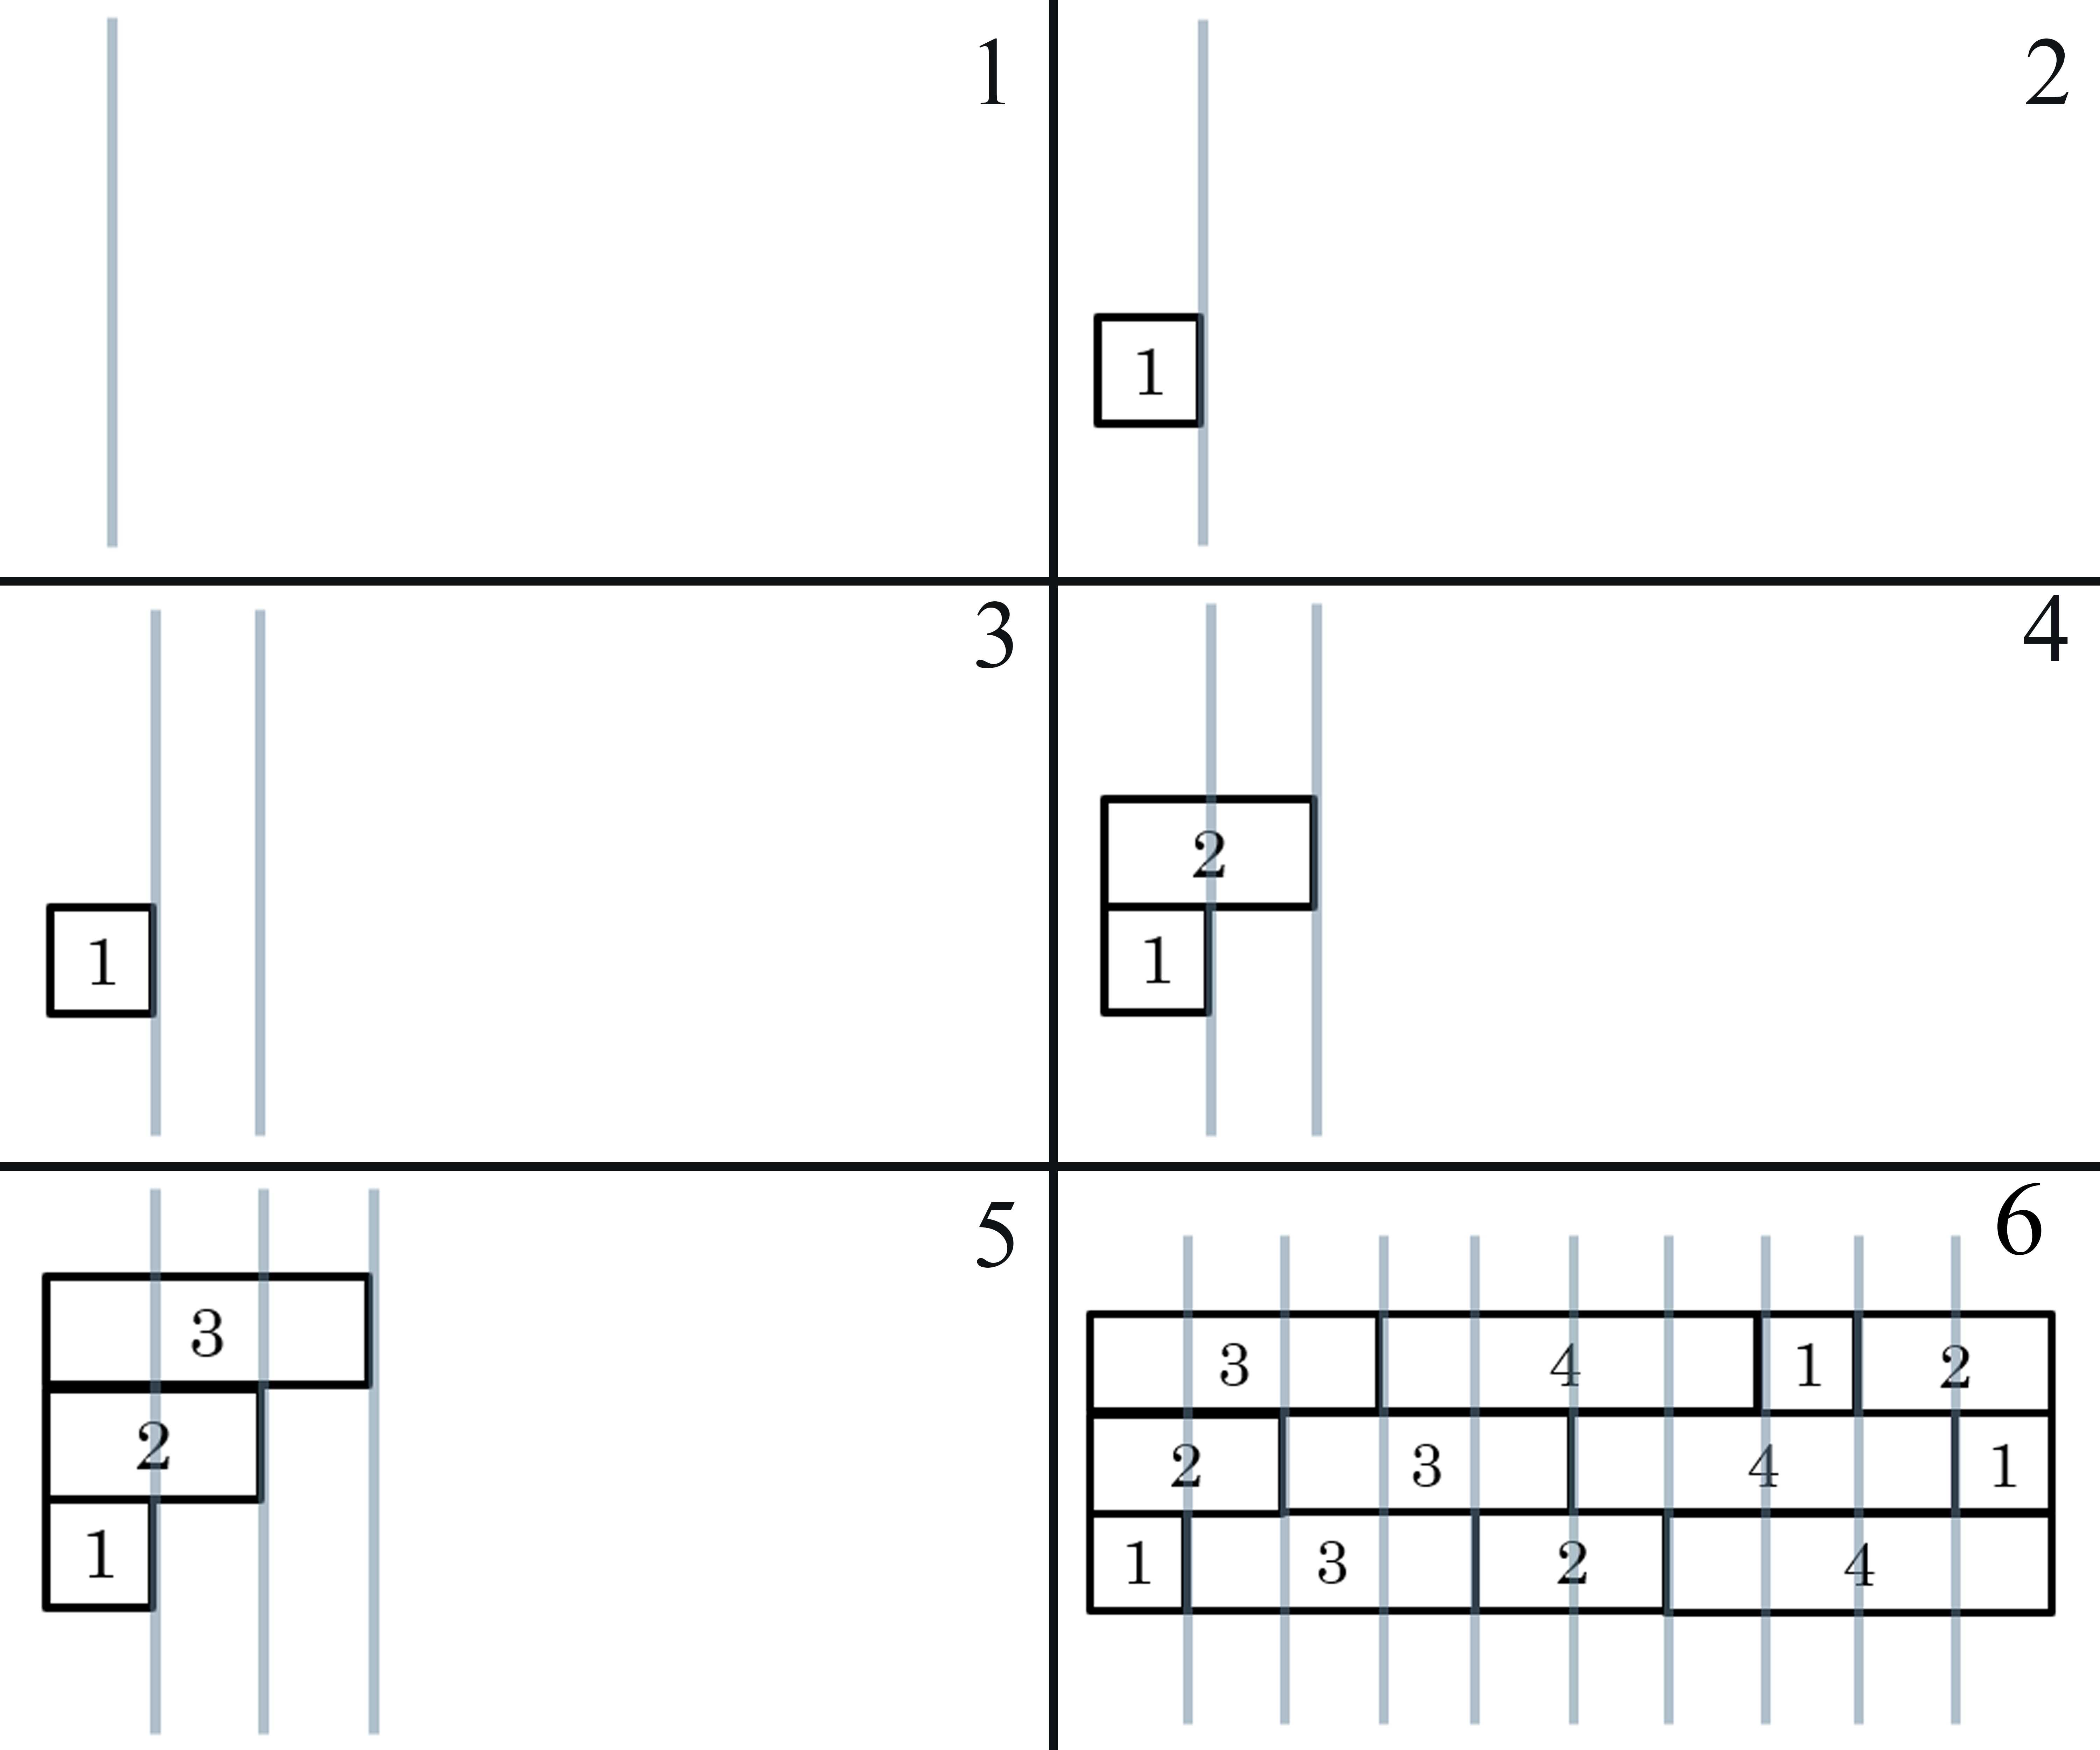
\includegraphics[width=1\linewidth]{Bilder/Aufgabe1/Definition_Mauerbauart_02.png}
    \caption{Der Bau einer Mauer nach der \textbf{„Von links nach rechts“}-Methode. Es wird jeweils immer die nächste freie Fuge angeschaut und überprüft, welches Klötzchen in welcher Reihe diese Fuge füllen kann. Dieses Klötzchen wird dann gesetzt (1 bis 5). Dies wiederholt sich so lange, bis die letzte Fuge erreicht wurde und die Mauer fertig ist (6).}
\end{figure}

Diese \textbf{„Von links nach rechts“}-Bauart ist dadurch möglich geworden, dass man schon von vornherein die Anzahl an Reihen kennt, die für eine maximale Mauer benötigt wird.

Aber auch bei dieser Bauart bleibt die Frage, was passiert, wenn mehr als ein Klötzchen die nächste Fuge füllen kann. Dies passiert nämlich bei fast jeder Fuge (siehe Abbildung 13).
\begin{figure}[H]
    \centering
    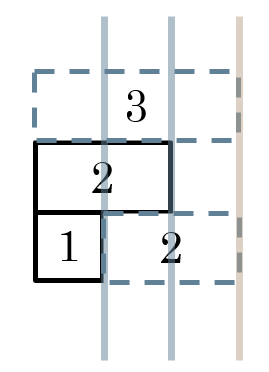
\includegraphics[width=0.3\linewidth]{Bilder/Aufgabe1/Problem_Mauerbauart_02_Mehrere_Kloetze.png}
    \caption{Zum Besetzen der dritten Fuge (orange markiert) bei $n = 4$ kann entweder ein 3er-Klötzchen in einer neuen Reihe, oder ein 2er-Klötzchen in der untersten Reihe platziert werden.}
\end{figure}

Wählt man ein zufälliges Klötzchen aus, so kann es schnell dazu kommen, dass eine Reihe so weit in „Rückstand“ gerät, dass kein mögliches Klötzchen mehr lang genug wäre, um die Reihe fortzuführen (siehe Abbildung 14).
\begin{figure}[H]
    \centering
    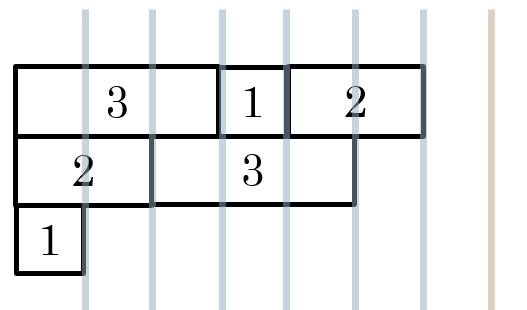
\includegraphics[width=0.5\linewidth]{Bilder/Aufgabe1/Problem_Mauerbauart_02_RowSum.png}
    \caption{In der dargestellten Mauer für $n = 4$ gibt es für die \textbf{unterste Reihe keine Möglichkeit mehr, ein Klötzchen zu platzieren}. Da die obereren Reihen alle Fugen schon besetzt haben und die nächste freie Fuge \textbf{6 Längen} von der untersten Reihe entfernt ist, würde diese Reihe ein \textbf{6er-Klötzchen} benötigen. Bei $n = 4$ gibt es jedoch maximal \textbf{4er-Klötzchen}.}
\end{figure}
Es ist also wichtig, immer darauf zu achten, dass die kürzeste Reihe nicht den Anschluss verliert.
\\[0.4cm]
Die Lösung für dieses Problem ist es, bei dem Fall, wenn verschiedene Klötzchen mehrerer Reihen eine Fuge befüllen können, immer die \textbf{kürzeste Reihe zu bevorzugen}.
\\[0.4cm]
Mit diesem Algorithmus kommt man bis zu $n = 8$. Dort tritt ein weiteres Problem auf (siehe Abbildung 15).
\begin{figure}[H]
    \centering
    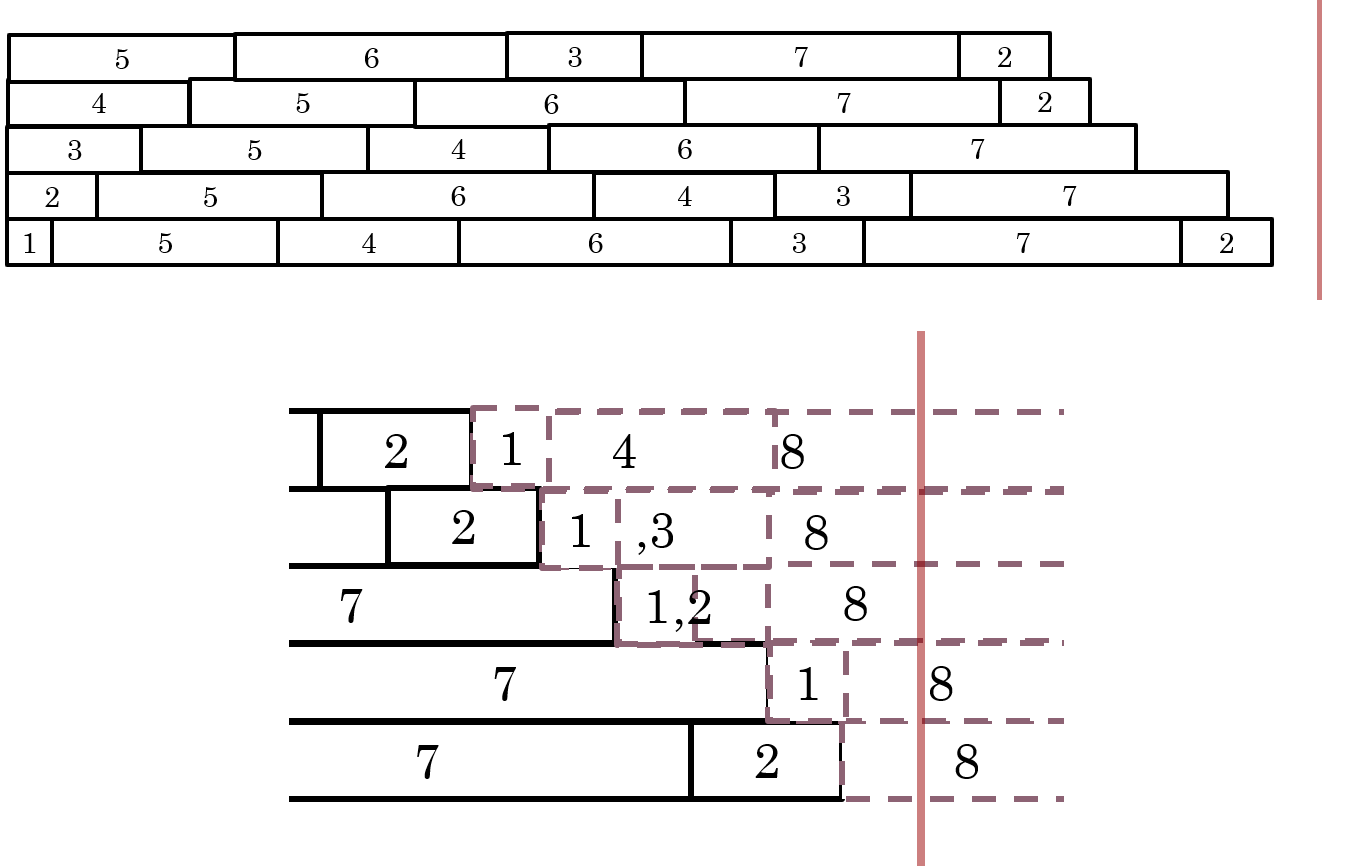
\includegraphics[width=1\linewidth]{Bilder/Aufgabe1/Problem_Mauerbauart_02_Kein_Klotz.png}
    \caption{Bei $n = 8$ tritt das Problem auf, dass die \textbf{29. Fuge} (rot markiert) durch \textbf{kein einziges mögliches Klötzchen besetzt werden kann}. Da $n$ jedoch eine \textbf{gerade Zahl} ist, wissen wir, dass für eine Mauer der maximalen Höhe \textbf{alle Fugen besetzt werden müssen}. Das untere Bild zeigt noch mal den hinteren Ausschnitt der Mauer mit allen noch möglichen Klötzchen für jede Reihe an. Keines davon würde die nächste Lücke füllen.}
\end{figure}
%TODO: Quelle für Backtracking
Um dennoch eine Lösung zu bekommen, wird \textbf{Backtracking} verwendet. Backtracking erlaubt es, \textbf{zur letzten Entscheidung zurückzugehen} und eben \textbf{eine andere} zu \textbf{treffen}. Mit „Entscheidung“ ist die Wahl eines Klötzchens, um eine freie Fuge zu besetzen, wenn es mehrere Möglichkeiten gibt, gemeint (siehe Abbildung 16).
\begin{figure}[H]
    \centering
    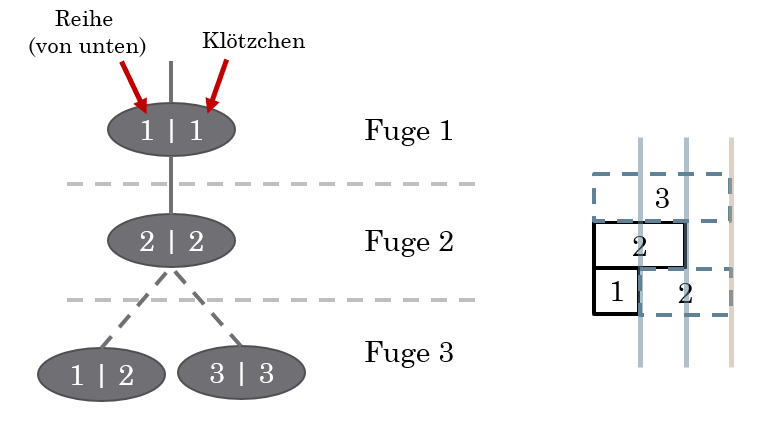
\includegraphics[width=1\linewidth]{Bilder/Aufgabe1/Backtracking_01.png}
    \caption{Bei einer Mauer von $n = 4$ tritt das vorher schon besprochene Problem auf, dass es zwei mögliche Klötzchen gibt, die die \textbf{3. Fuge} besetzen können. Der Baum auf der linken Seite veranschaulicht die möglichen Klötzchen pro Fuge. Die \textbf{Tiefe des Baumes} entspricht dabei einer \textbf{jeweiligen Fugenposition} und die \textbf{Knoten dieser Tiefe} stehen für die \textbf{möglichen Klötzchen}.}
\end{figure}
Nun wird das Klötzchen der kürzesten Reihe (das 3er-Klötzchen in der obersten, neuen Reihe) gewählt und \textbf{davon ausgegangen, dass die 4. Fuge danach nicht mehr gefüllt werden kann} (siehe Abbildung 17).
\begin{figure}[H]
    \centering
    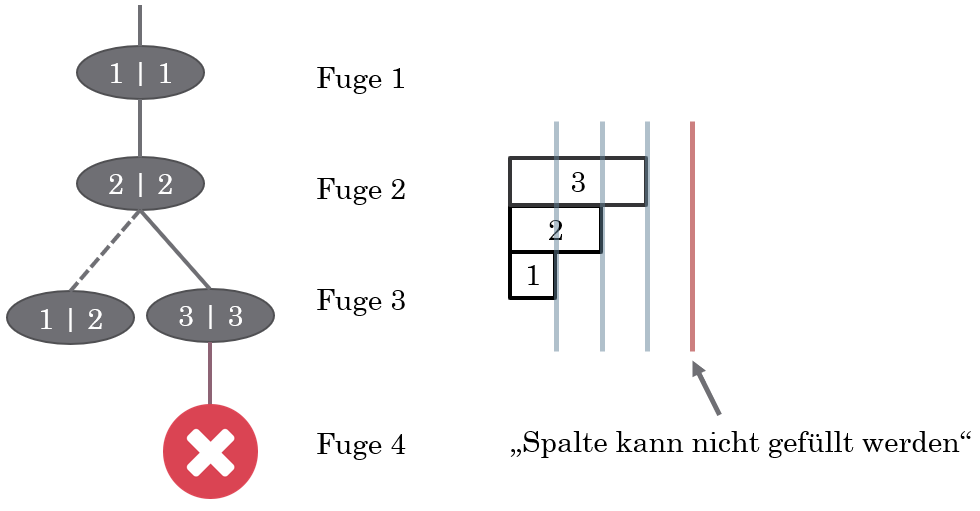
\includegraphics[width=1\linewidth]{Bilder/Aufgabe1/Backtracking_02.png}
    \caption{Angenommen, nach der Entscheidung, das 3. Klötzchen einzusetzen, kann die 4. freie Fuge nicht besetzt werden. Theoretisch könnte in der untersten Reihe ein 3er-Klötzchen die 4. Fuge füllen. Zur Vereinfachung der Darstellung wird dies jedoch außer Acht gelassen.}
\end{figure}
Daraufhin wird \textbf{einen Schritt zurück zur letzten Entscheidung} gegangen und \textbf{dort das andere Klötzchen} gewählt (siehe Abbildung 18).
\begin{figure}[H]
    \centering
    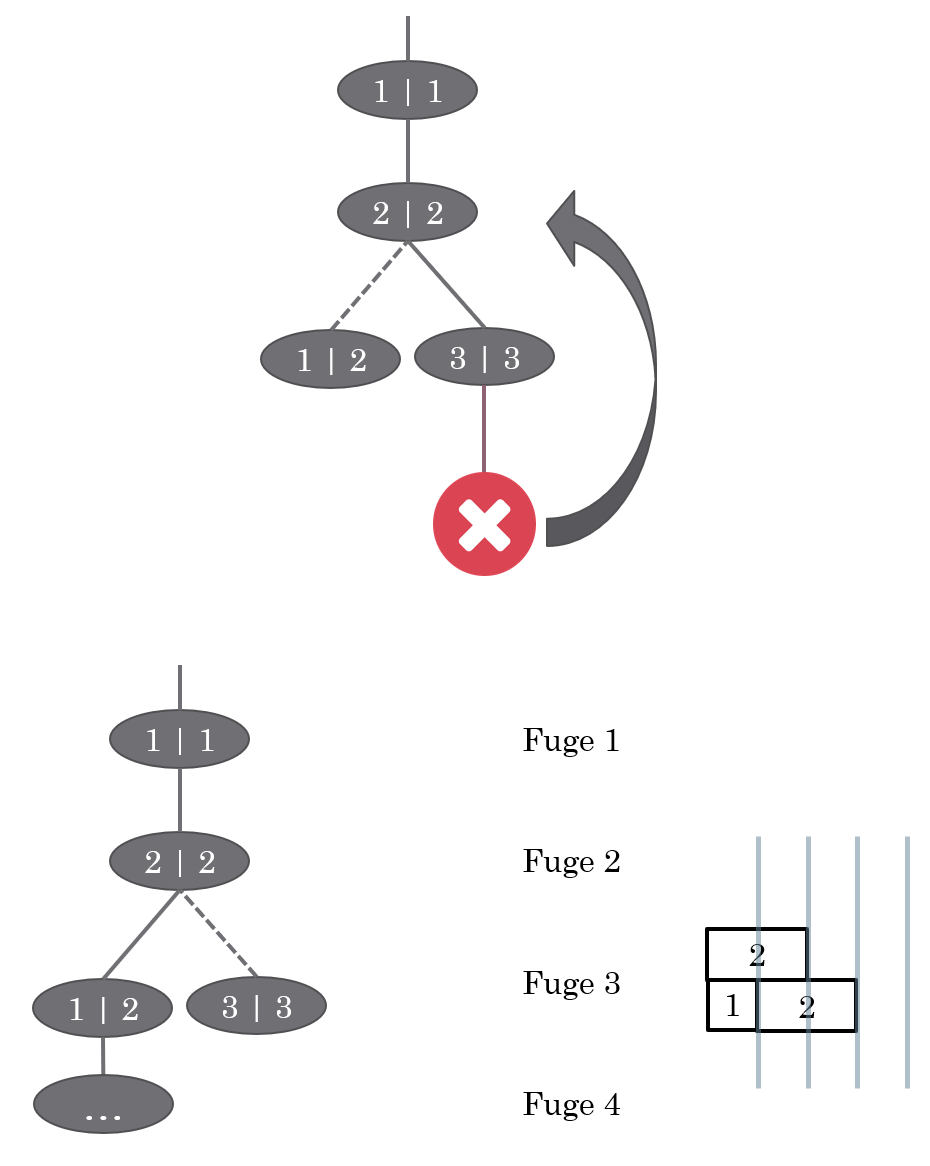
\includegraphics[width=1\linewidth]{Bilder/Aufgabe1/Backtracking_03_04.png}
    % TODO: Quelle für Trial and error Prinzip
    \caption{Nach dem „Trial and error“-Prinzip wird beim Backtracking zur letzten Entscheidung zurückgegangen (oberes Bild) und ein anderes Klötzchen ausgewählt (unteres Bild). Dann wird mit dem Algorithmus fortgefahren.}
\end{figure}

Damit ist der grundlegende Algorithmus vollständig.
\subsection{Implementierung}
Das Programm wurde in der Sprache C\# als Konsolen-Applikation mit dem .NET Framework 4.7.1 geschrieben.
Das am Ende des Kapitels in Abbildung 21 stehende Klassendiagramm zeigt die Grundstruktur des Programms.
\\[0.4cm]
Im Folgenden soll nur die Implementierung der für den „Von links nach rechts“-Algorithmus wichtigsten Methode erklärt werden. Auf der beigelegten CD befindet sich zusätzlich eine vollständige Dokumentation aller Methoden und Attribute einmal in Form eines PDFs und einer HTML-Website.
\\[0.4cm]
Die Klasse \code{WallBuilder} ist für den Algorithmus die wichtigste Klasse. Sie baut die Mauer. Die für diesen Vorgang verantwortliche Methode ist \code{FillNextGap} (siehe Abbildung 20), die als Eingabeparameter einen Integer \code{nextGap}, ein \code{Wall} Objekt \code{curWall} und einen weiteren Integer \code{freeGaps} erwartet und ein Objekt der Klasse \code{Wall} zurückgibt.
\\[0.4cm]
Die Methode ist \textbf{direkt rekursiv} und teilt somit die Problemstellung, eine komplette Mauer zu bauen, in mehrere kleinere Probleme auf. Diese sind, für die jeweils nächste Fuge ein Klötzchen zu finden, das sie besetzt.
\\[0.4cm]
% TODO: Quelle für LINQ
Als Erstes wird mit der Abbruchbedingung in Zeile 4 kontrolliert, ob die Mauer vollständig gebaut ist. Durch das Programmiermodell \textbf{LINQ} wird überprüft, ob die Summe aller platzierten Klötzchen jedes \code{Row} Objekts der übergebenen \code{Wall} Instanz \code{curWall} mit der Länge einer vollständigen Mauer übereinstimmt.
Ist die Abbruchbedingung \code{true}, so kommt es zu einem Rekursionsende und das fertige \code{Wall} Objekt wird zurückgegeben.
\\[0.4cm]
% TODO: Quelle für Reference-Type
Ansonsten wird das übergebene \code{Wall} Objekt „kopiert“, denn es ist sehr wichtig, dass am übergebenen \code{curWall} Objekt nichts geändert wird. Objekte der Klassen \code{Wall} und \code{Row} sind nämlich sogenannte Referenz-Typen (engl. Reference Types). Anders als bei Werte-Typen (engl. Value Types), bei denen bei einer erneuten Zuweisung der gespeicherte Wert kopiert und die Variable dann auf diesen kopierten Wert verweist, wird bei einer erneuten Zuweisung eines Referenz-Typs \textbf{nur der Verweis} (engl. Pointer) \textbf{kopiert}. Die Variable greift jedoch auf das \textbf{gleiche Objekt im Systemspeicher} zu wie die vorherige Variable.

Dies hätte zur Folge, dass wenn an dem übergebenen \code{Wall} Objekt zu späterem Zeitpunkt irgendwelche Änderungen vorgenommen werden, sich auch das \code{Wall} Objekt der Aufrufer-Methode ändert. Dies würde das Backtracking erheblich erschweren, da nicht mehr auf den Zustand der Mauer \textbf{vor einer Klötzchen-Entscheidung} zurückgegriffen werden könnte.
\\[0.4cm]
In Zeile 10 bis 14 wird dann die für den aktuellen Schritt zu befüllende Fugenposition gewählt. Der Parameter \code{nextGap} beschreibt also die \textbf{zuletzt gefüllte Fuge}.

Es wird überprüft, ob es nach \code{nextGap} überhaupt noch eine Fuge gibt. Ist dem so, wird die Variable \code{nextGapPos} mit dem Wert \code{nextGap + 1}, also der Position der nächsten Fuge, initialisiert. Es kann jedoch auch sein, dass die Mauer schon am Ende angelangt ist und im letzten Schritt bereits die letzte „Fugenposition“ und damit ist hierbei das Ende der Mauer gemeint, gefüllt wurde (siehe Abbildung 19). Wichtig ist, dass dies nicht direkt heißt, dass die Mauer fertig ist. Es muss nämlich jede andere Reihe auch noch die letzte „Fuge“ erreichen.
\begin{figure}[H]
    \centering
    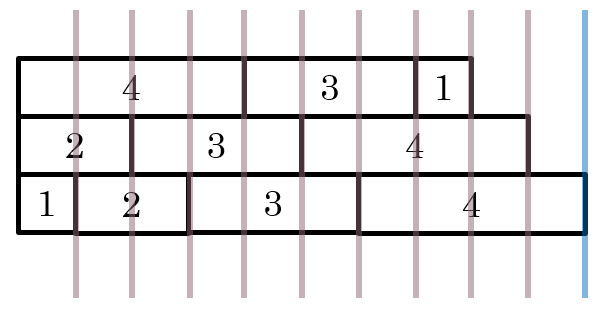
\includegraphics[width=.6\linewidth]{Bilder/Aufgabe1/Code_Algorithmus_01.png}
    \caption{Bei dieser Mauer von $n = 4$ hat die unterste Reihe die letzte „Fugenposition“ bereits gefüllt. Diese End-„Fuge“ darf und muss jedoch mehrmals besetzt werden, um jede Reihe abzuschließen.}
\end{figure}
Deshalb wird in diesem Fall die Variable \code{nextGapPos} mit dem gleichen Wert wie \code{nextGap} initialisiert.
\\[0.4cm]
% TODO: QUELLE für LINQ
Im nächsten Ausdruck, der sich von Zeile 17 bis 19 erstreckt, werden wieder mittels \textbf{LINQ} alle \code{Row} Objekte der aktuellen \code{Wall} Instanz, die durch ein noch verfügbares Klötzchen die gewünschte Fugenposition befüllen können, in einem Array gesammelt.
\\[0.4cm]
Von Zeile 22 bis 34 wird nun geprüft, ob es keine einzige Reihe gibt, die die nächste Fuge besetzen kann. Hier wird der Sonderfall berücksichtigt, dass der Parameter \code{freeGaps} größer als 0 ist. Dies kann nämlich der Fall sein, wenn $n$ \textbf{ungerade} ist. Bei ungeraden $n$ kann es ja zu vollständigen Mauern kommen, \textbf{ohne}, dass \textbf{alle} Fugen besetzt sind. In der Tat kann man auch relativ einfach ausrechnen, wie viele Fugen für ein ungerades $n$ frei bleiben können (siehe Methode \code{CalculateWallProperties} der Klasse \code{WallBuilder}. Somit kann es passieren, wenn kein Klötzchen in keiner Reihe zum Besetzen einer freien Fuge gefunden wurde und der „freie Fugen-Puffer“ der aktuellen Mauer noch größer als 0 ist, dass diese freie Fuge \textbf{nicht besetzt} und einfach \textbf{übersprungen} werden kann.
Deshalb findet in Zeile 26, wenn \code{freeGaps} noch größere als 0 ist, einfach der rekursive Aufruf statt, mit dem \code{freeGaps} Parameter um 1 verringert. Der Rückgabewert dieses rekursiven Aufrufs wird in der Variable \code{result} gespeichert. Ist \code{result} ein \code{Wall} Objekt, wird dieses weiter zurückgegeben, ansonsten wird der restliche Code bis zum Rekursionsende in Zeile 51 ausgeführt.
Tritt der Sonderfall \code{freeGaps > 0} nicht ein wird \code{null} zurückgegeben.
\\[0.4cm]
In Zeile 37 wird das Array der \code{Row} Objekte, die die nächste Fuge füllen können, nach ihrer \code{RowSum} sortiert. Mit \code{RowSum} ist hierbei einfach die Summe aller in der Reihe platzierten Klötzchen gemeint.
Nach dem Sortieren ist das erste Objekt des \code{possibleRows} Arrays also die \textbf{kürzeste Reihe} und das letzte Objekt die bereits \textbf{längste Reihe}.
\\[0.4cm]
In der For-Schleife von Zeile 40 bis 48 werden nun die \code{Row} Objekte des \code{possibleRows} Array einzeln iteriert.
Zuerst wird in Zeile 42 das Klötzchen platziert, das die gesuchte Fuge füllt. (Das Klötzchen wurde in der vorher aufgerufenen Methode \code{ContainsPossibleRowSum} der Klasse \code{WallBuilder} herausgefiltert.)

Danach kommt ein rekursiver Aufruf, dessen Rückgabewert in der lokalen Variabel \code{result} gespeichert wird. In der Abbruchbedingung von Zeile 44 wird wieder überprüft, ob \code{result} ein \code{Wall} Objekt ist. Ist dies der Fall, wird es weiter zurückgegeben.

Ist im Gegensatz dazu \code{result} gleich \code{null}, heißt das, dass mit dieser Klötzchen-Entscheidung keine fertige Mauer gebaut werden konnte und deshalb bis zu dieser Entscheidung zurückgegangen wurde, um dort ein anderes Klötzchen zu wählen (\textbf{Backtracking}).

Deshalb wird das zuvor platzierte Klötzchen des aktuellen \code{Row} Objekts in Zeile 47 wieder entfernt.

Gibt es danach noch weitere \code{Row} Objekte im \code{possibleRows} Array, wird die Schleife mit dem nächsten \code{Row} Objekt durchlaufen.
\\[0.4cm]
Als letzte Anweisung der Methode wird mit einem Rekursionsende \code{null} zurückgegeben.
\begin{figure}[H]
    \centering
    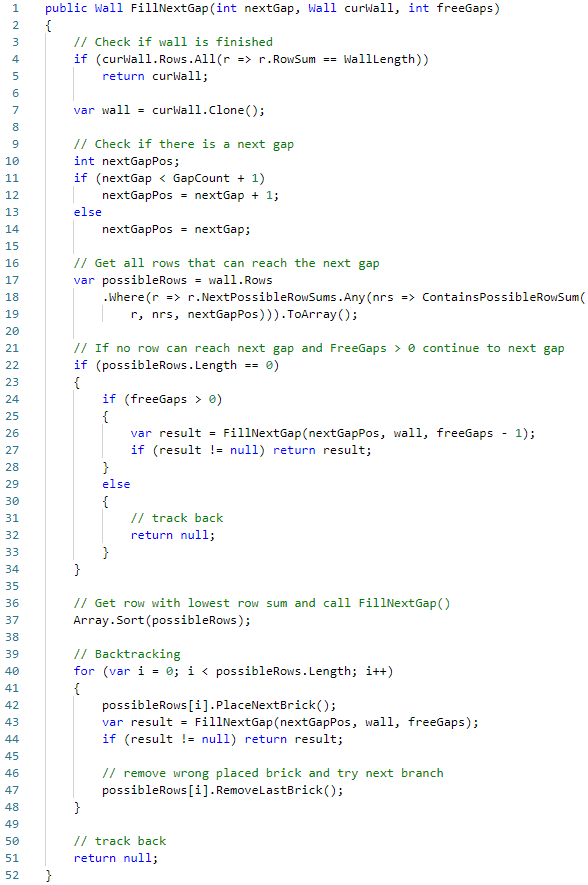
\includegraphics[width=.86\linewidth]{Bilder/Aufgabe1/Code.png}
    \caption{Quellcode der Methode \code{FillNextGap} der Klasse \code{WallBuilder}}
\end{figure}
\begin{figure}[H]
    \centering
    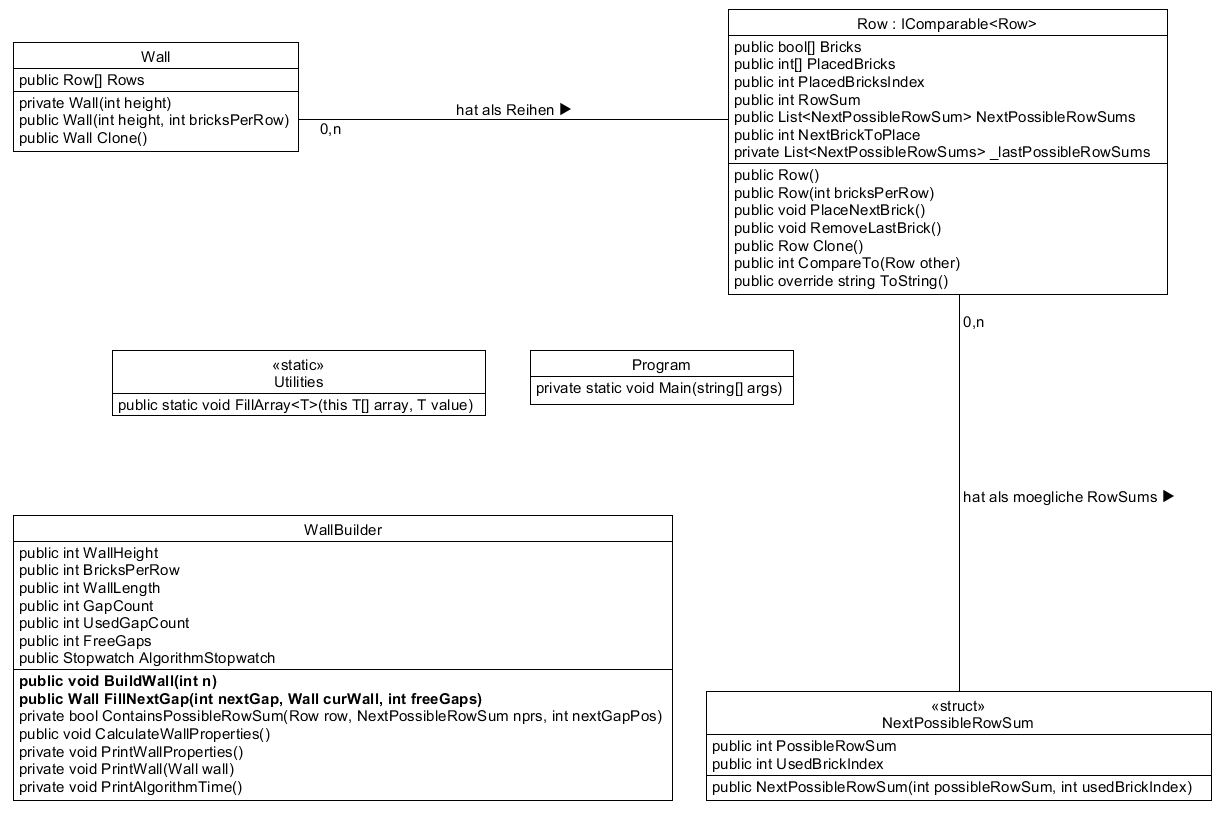
\includegraphics[width=.925\linewidth]{Bilder/Aufgabe1/Klassendiagramm.png}
    \caption{Erweitertes Klassendigramm des Programms. Die wichtigsten zwei Methoden des Algorithmus wurden in der Klasse \code{WallBuilder} hervorgehoben.}
\end{figure}

\subsection{Optimierungsmöglichkeiten}
Mit der Implementierung dieses Algorithmus können maximale Mauern bis zu $n = 17$ in wenigen Sekunden erzeugt werden. Jedoch steigt die durchschnittliche Algorithmuslaufzeit ab $n = 17$ sehr stark an. Für $n = 18$ dauert das Finden einer Mauer schon mehrere Minuten.
\\[0.4cm]
% TODO: QUELLE FÜR BWINF LÖSUNGEN
Dieser Algorithmus lässt sich jedoch noch wesentlich optimieren. In den vom Bundeswettbewerb Informatik offiziell veröffentlichten Lösungshinweisen werden zur ersten Aufgabe noch mehrere Optimierungsmöglichkeiten genannt:
\begin{itemize}
\item Randomized Algorithm
\item Kopplung und Spiegelung einer halben Mauer
\item Einschränkung des Suchraums
\item Ergänzung vorheriger Permutationen
\end{itemize}

Mithilfe dieser Optimierungen kann der Algorithmus so erweitert werden, dass er bis $n = 110$ eine Mauer wenigen Minuten generieren kann.

Dies ist vor allem eindrucksvoll, wenn man bedenkt, dass es für $n = 100$ schon
\begin{center}
\begin{Large}
\[100!^{51} \approx 2,95\mathrm{e}{+8,056}\]
\end{Large}
\end{center}
unterschiedliche Mauern der maximalen Höhe gibt.

Das ist eine Zahl mit \textbf{8057 Stellen}.

\subsection{Beispiele}
Wie bereits erwähnt, kann der Algorithmus Mauern von $n = 2$ bis $n = 17$ in wenigen Sekunden erstellen. Weitere Test mit größeren $n$ wurden nach mehreren Minuten abgebrochen.
\\[0.4cm]
Außerdem können Mauern von $n = 2$ bis $n = 7$ komplett \textbf{ohne Backtracking} generiert werden. Dies sorgt dafür, dass die Algorithmuslaufzeiten für diese $n$ in etwa gleich sind.
\\[0.4cm]
Weiterhin erwähnenswert ist, dass das Finden von Mauern für ungerade $n$ meist kürzer dauert als das Generieren der $n - 1$ Mauer, da dort Fugen freigelassen werden können und es dadurch deutlich mehr mögliche Mauerkombinationen gibt.
\\[0.4cm]
Im Folgenden sind die durchschnittlichen Algorithmuslaufzeiten für die verschiedenen $n$ in einer Tabelle aufgelistet.
\vspace{0.4cm}
\begin{table}[H]
\begin{center}
\begin{tabular}{cr}
\hline
n  & Algorithmuslaufzeit \\ \hline
2  & 10,25 ms            \\
3  & 10 ms               \\
4  & 11 ms               \\
5  & 10 ms               \\
6  & 10,75 ms            \\
7  & 10,75 ms            \\
8  & 10 ms               \\
9  & 10,75 ms            \\
10 & 15 ms               \\
11 & 14,75 ms            \\
12 & 29,25 ms            \\
13 & 42 ms               \\
14 & 372 ms              \\
15 & 125 ms              \\
16 & 11348 ms            \\
17 & 636 ms             
\end{tabular}
\end{center}
\end{table}

Die linke Spalte gibt den eingegeben Wert für $n$ an, die rechte die durchschnittliche Algorithmuslaufzeit in Millisekunden.
\\[0.4cm]
Außerdem zeigen Abbildung 22 bis 24 Konsolen-Ausgaben des Programms für verschiedene $n$.
Die Mauerlösung ist dabei die hellblaue Ausgabe. Die verschiedenen Klötzchen einer Reihe werden mit dem Trennstrich (\code{|}) abgetrennt. Die Zahl innerhalb der Trennstriche steht für die Länge eines Klötzchens.
\begin{figure}[H]
    \centering
    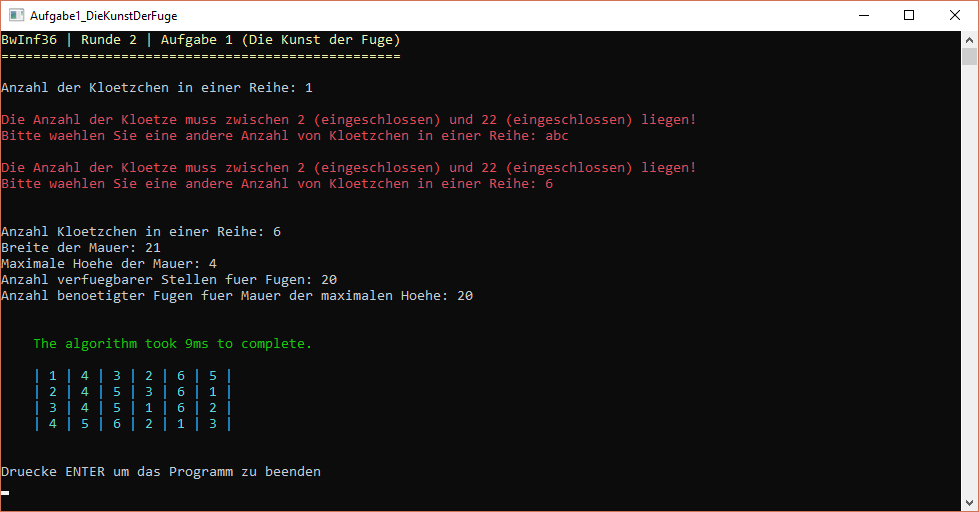
\includegraphics[width=1\linewidth]{Bilder/Aufgabe1/Programm_6.png}
    \caption{Programm-Ausgabe für $n = 6$ mit vorherigen fehlerhaften Eingaben für $n$ (1 und abc)}
\end{figure}
\begin{figure}[H]
    \centering
    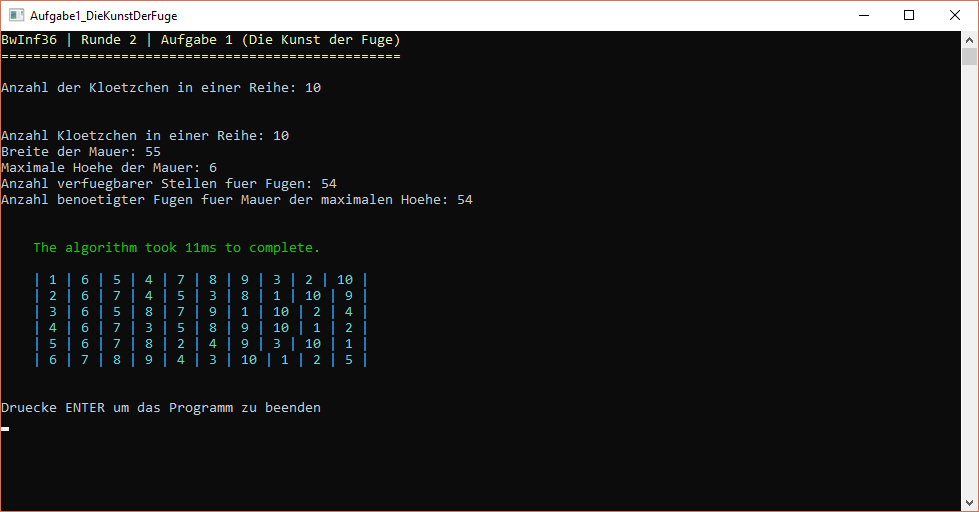
\includegraphics[width=1\linewidth]{Bilder/Aufgabe1/Programm_10.png}
    \caption{Programm-Ausgabe für $n = 10$}
\end{figure}
\begin{figure}[H]
    \centering
    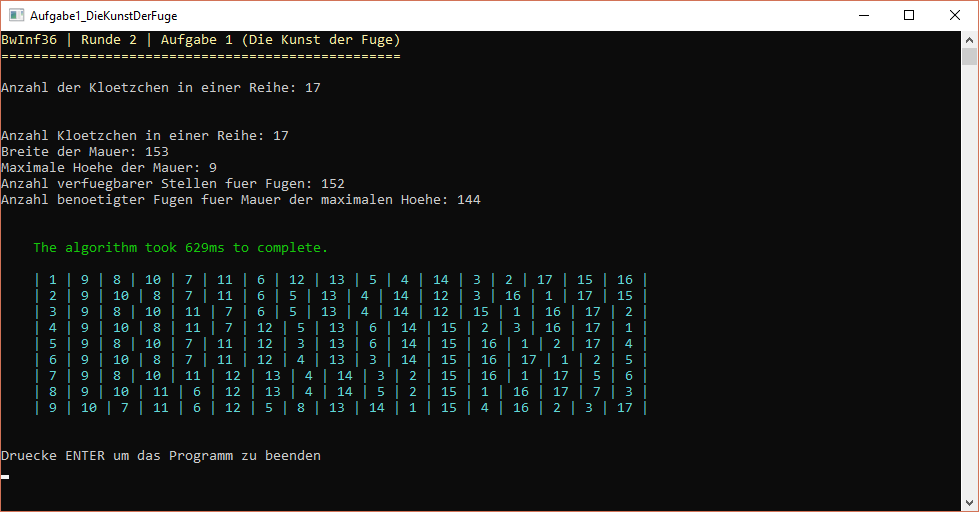
\includegraphics[width=1\linewidth]{Bilder/Aufgabe1/Programm_17.png}
    \caption{Programm-Ausgabe für $n = 17$}
\end{figure}





%===================================================================================
%-------------------------------- AUFGABE 3 ----------------------------------------
%===================================================================================

\newpage
\section{AUFGABE 3 – „Quo vadis, Quax?“}



\subsection{Aufgabenstellung}
In einer abgelegenen und unwegsamen Gegend will Quax die Fähigkeiten seines neuen Quadcopters
ausprobieren. Da wird aus dem Spiel Ernst: Ein Tornado mit anschließender Überschwemmung
vernichtet seine Essenvorräte, so dass er seinen Urlaub abbrechen und sofort die
lange Wanderung zurück zur einzigen Stadt der Provinz antreten muss. Außerdem hat sich die
Landschaft vollkommen verändert – es haben sich Flüsse und Seen gebildet, wo früher keine
waren. Es ist nicht klar, ob es überhaupt noch einen gangbaren Weg zurück zur Stadt gibt und,
falls ja, wo sich ein solcher Weg zwischen den Gewässern durchschlängelt.
\\[0.4cm]
Quax möchte die Landschaft mit dem Quadcopter erkunden, bevor er loslegt, um lange Umwege
zu vermeiden, die er sich nicht leisten kann. Der Quadcopter kann in einer frei wählbaren
Flughöhe einen beliebigen Punkt der Landschaft anfliegen. Allerdings ist auch er beschädigt:
Die Speicherkarte ist hin, und es funktioniert nur ein einziger Sensor. Dieser erfasst ein quadratisches,
nach Norden ausgerichtetes Gebiet unter dem Quadcopter, dessen Seitenlänge proportional
zur Flughöhe ist. Der Sensor kann für dieses Testgebiet entscheiden, ob es ganz von
Wasser bedeckt ist („Wasser“), ganz aus trockenem Land besteht („Land“) oder sowohl Wasser
als auch Land enthält („Gemischt“).
\\[0.4cm]
Quax kann wiederholt den Quadcopter für eine bestimmte Kombination aus Flughöhe und Zielpunkt
programmieren, ihn entsenden und bei seiner Rückkehr das Ergebnis („Wasser“, „Land“
oder „Gemischt“) in Empfang nehmen. Liefert der Quadcopter auch für ein kleinstmögliches
Testgebiet mit Seitenlänge 20m immer noch das Ergebnis „Gemischt“, geht Quax davon aus,
dass er dieses Testgebiet überqueren kann – zur Not schwimmt er ein paar Meter mit dem Gepäck.
\\[0.4cm]
Das folgende Pixelbild zeigt eine Beispiel-Landschaft. Jedes Pixel repräsentiert einen quadratischen
Bereich der Landschaft mit Seitenlänge 10 m. Das grüne Pixel zeigt die Position der
Stadt. Vom oberen roten Startpunkt kann Quax die Stadt erreichen, vom unteren aber nicht.
\begin{figure}[H]
\centering
    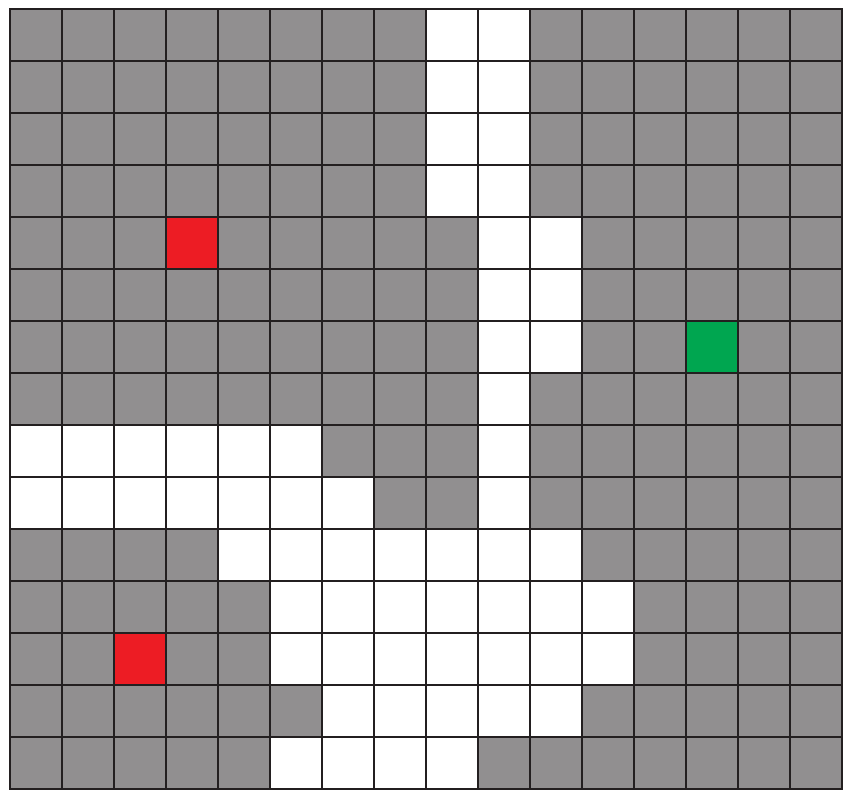
\includegraphics[width=0.4\linewidth]{Bilder/Aufgabe3/Aufgabenstellung_01.png}
\end{figure}
\begin{large}
    \textbf{Aufgabe} \\
\end{large}
\vspace{-0.6cm}
\begin{enumerate}[label=(\emph{\alph*})]
\item Schreibe ein Programmmodul, das aus den Ergebnissen durchgeführter Flüge bestimmt,
ob es für Quax einen gangbarenWeg zurück zur Stadt gibt, ob es definitiv keinen solchen
Weg gibt oder ob mehr Flüge nötig sind, um eine Entscheidung herbeizuführen.
\item Beschreibe eine Strategie für das Entsenden des Quadcopters, die mit möglichst wenig
Flügen einen Weg zur Stadt findet, falls es einen gibt.
\item Schreibe ein Programm, das eine Landschaft einliest, in welcher die Stadt sowie mehrere
mögliche Standorte von Quax markiert sind. Ein Pixel repräsentiert ein Quadrat der
Seitenlänge 10 m. Dann soll das Programm die anhand der Strategie aus (b) festgelegten
Entsendungen – für jeden Standort des Quadcopters einzeln – simulieren. Ausgeben soll
es je eine Darstellung der Landschaft, in der die Testgebiete mit ihren jeweiligen Ergebnissen
geeignet eingetragen sind. Falls es einen gangbaren Weg zur Stadt gibt, soll dieser
in der Darstellung erkennbar sein.

Wende dein Programm mindestens auf die auf der BWINF-Website gegebenen Beispiele
an und dokumentiere die Ergebnisse. Gehe davon aus, dass sich außerhalb der eingelesenen
Landschaft nur Wasser befindet.
\item Gibt es Verteilungen von Flüssen und Seen, bei denen deine Strategie aus (b) zu sehr
vielen Flügen führt? Falls nein, erkläre warum nicht. Falls ja, gib ein Beispiel dafür an
und erkläre, worin das Problem besteht.
\end{enumerate}

\subsection{Auslegung der Aufgabe}
Die Aufgabenstellung ist größtenteils sehr klar. Das grundlegende Problem ist eine Wegfindung. Jedoch reicht als Lösung kein einfacher Wegfindungs-Algorithmus, da es bestimmte Bedingungen gibt, wie das der Quadcopter minimal 20x20 Gebiete scannen kann. Beim Scannen eines Gebiets gibt es 3 Mögliche Resultate. Entweder das Gebiet besteht eindeutig aus Wasser oder aus Land, oder das Gebiet liefert den Wert gemischt und besitzt damit sowohl Wasser als auch Land.

Das Endziel des Algorithmus ist nicht wie bei den meisten normalen Pathfinding Algorithmen möglichst schnell einen möglichst kurzen Weg zu finden, sondern mit \textbf{möglichst wenig Flügen} einen Pfad zur Stadt zu finden.

Angenommen man verwendet einen auf einem 20x20 Gitter basierenden Wegfindungs-Algorithmus, so müsste der Quadcopter zuerst
\begin{center}
\begin{Large}
\[\lceil \frac{w}{2}\rceil \times \lceil \frac{h}{2}\rceil\]
\end{Large}
\end{center}
wobei $w$ die Breite und $h$ die Höhe der Karte sind, Flüge durchführen, um das benötigte Gitter zu erstellen.
Im Falle der ersten offiziellen Test-Map des BwInfs (siehe Abbildung 25) mit den Dimensionen 1674x1102 wären das \textbf{461,187 Flüge}.
\begin{figure}[H]
\centering
    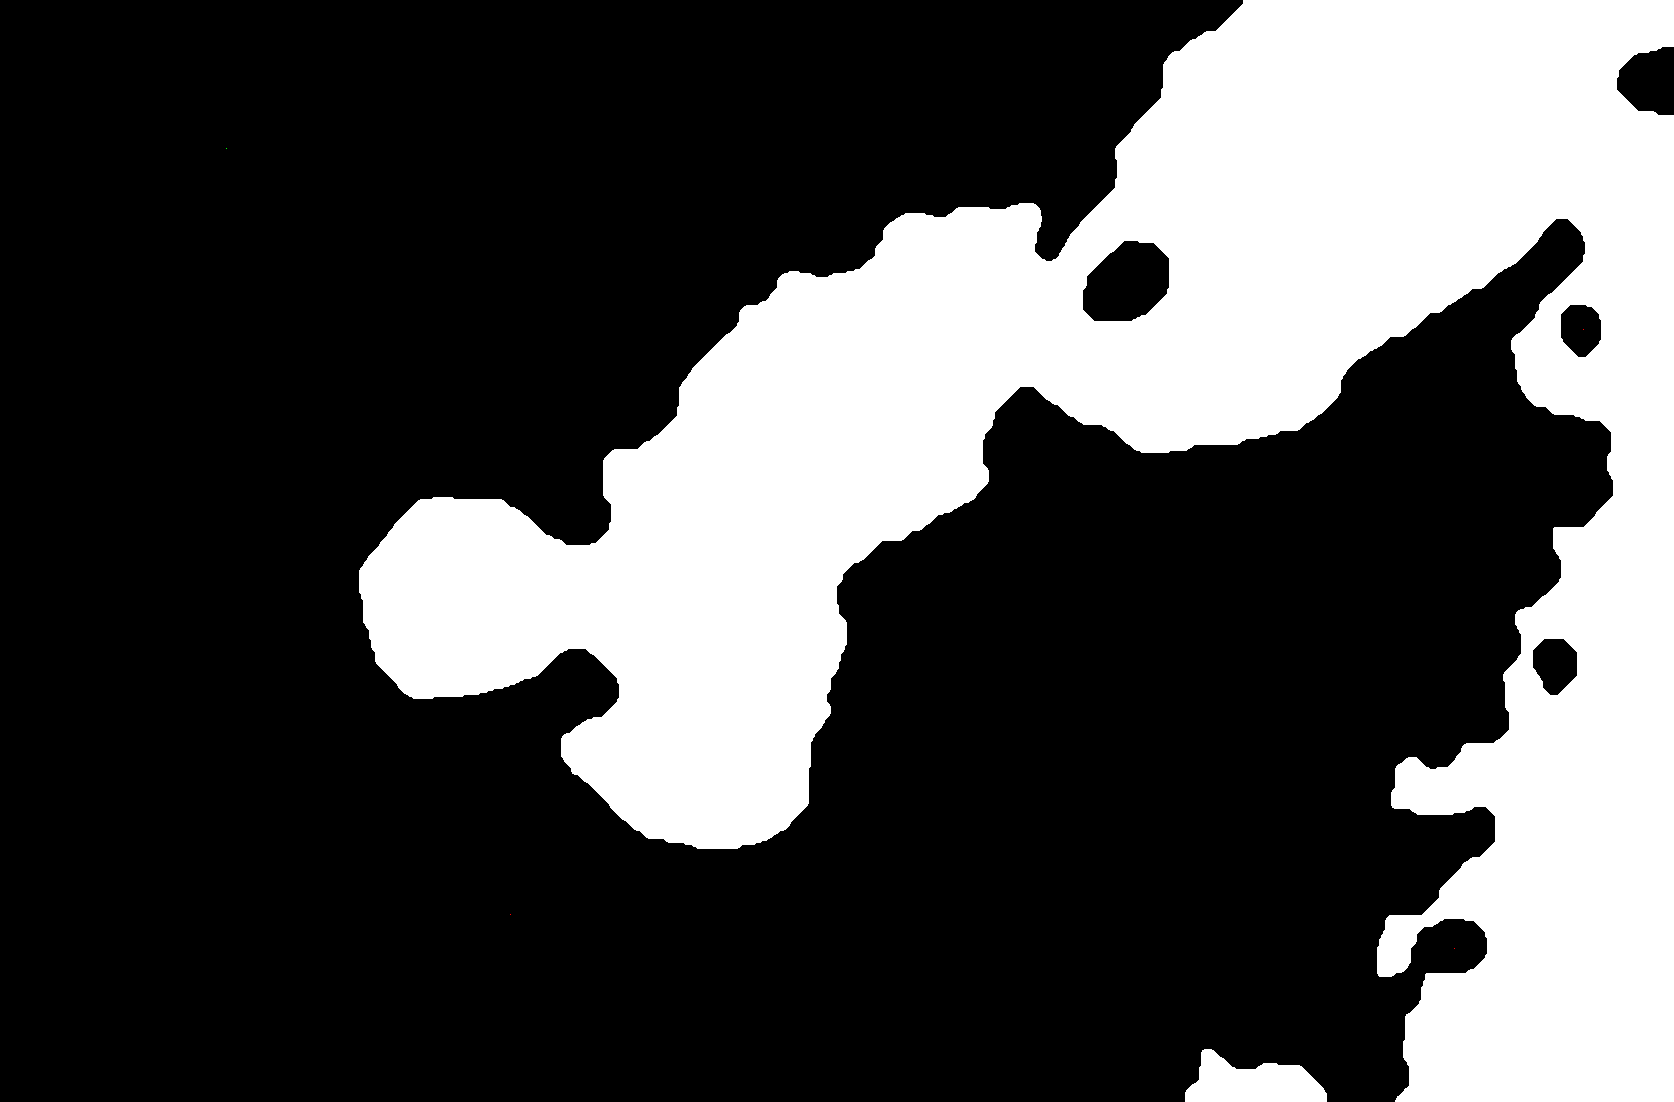
\includegraphics[width=0.8\linewidth]{Bilder/Aufgabe3/Maps/quax1.png}
    \caption{quax1.png des zur Aufgabe 3 verfügbar gestellten Materials}
\end{figure}
Hier könnte man allerdings allein schon zehntausende Flüge einsparen, wenn man den Quadcopter die linke obere Ecke von einer höheren Position aus scannen lasst, so dass er ein größeres Gebiet auf einmal betrachtet (siehe Abbildung 26).
\begin{figure}[H]
\centering
    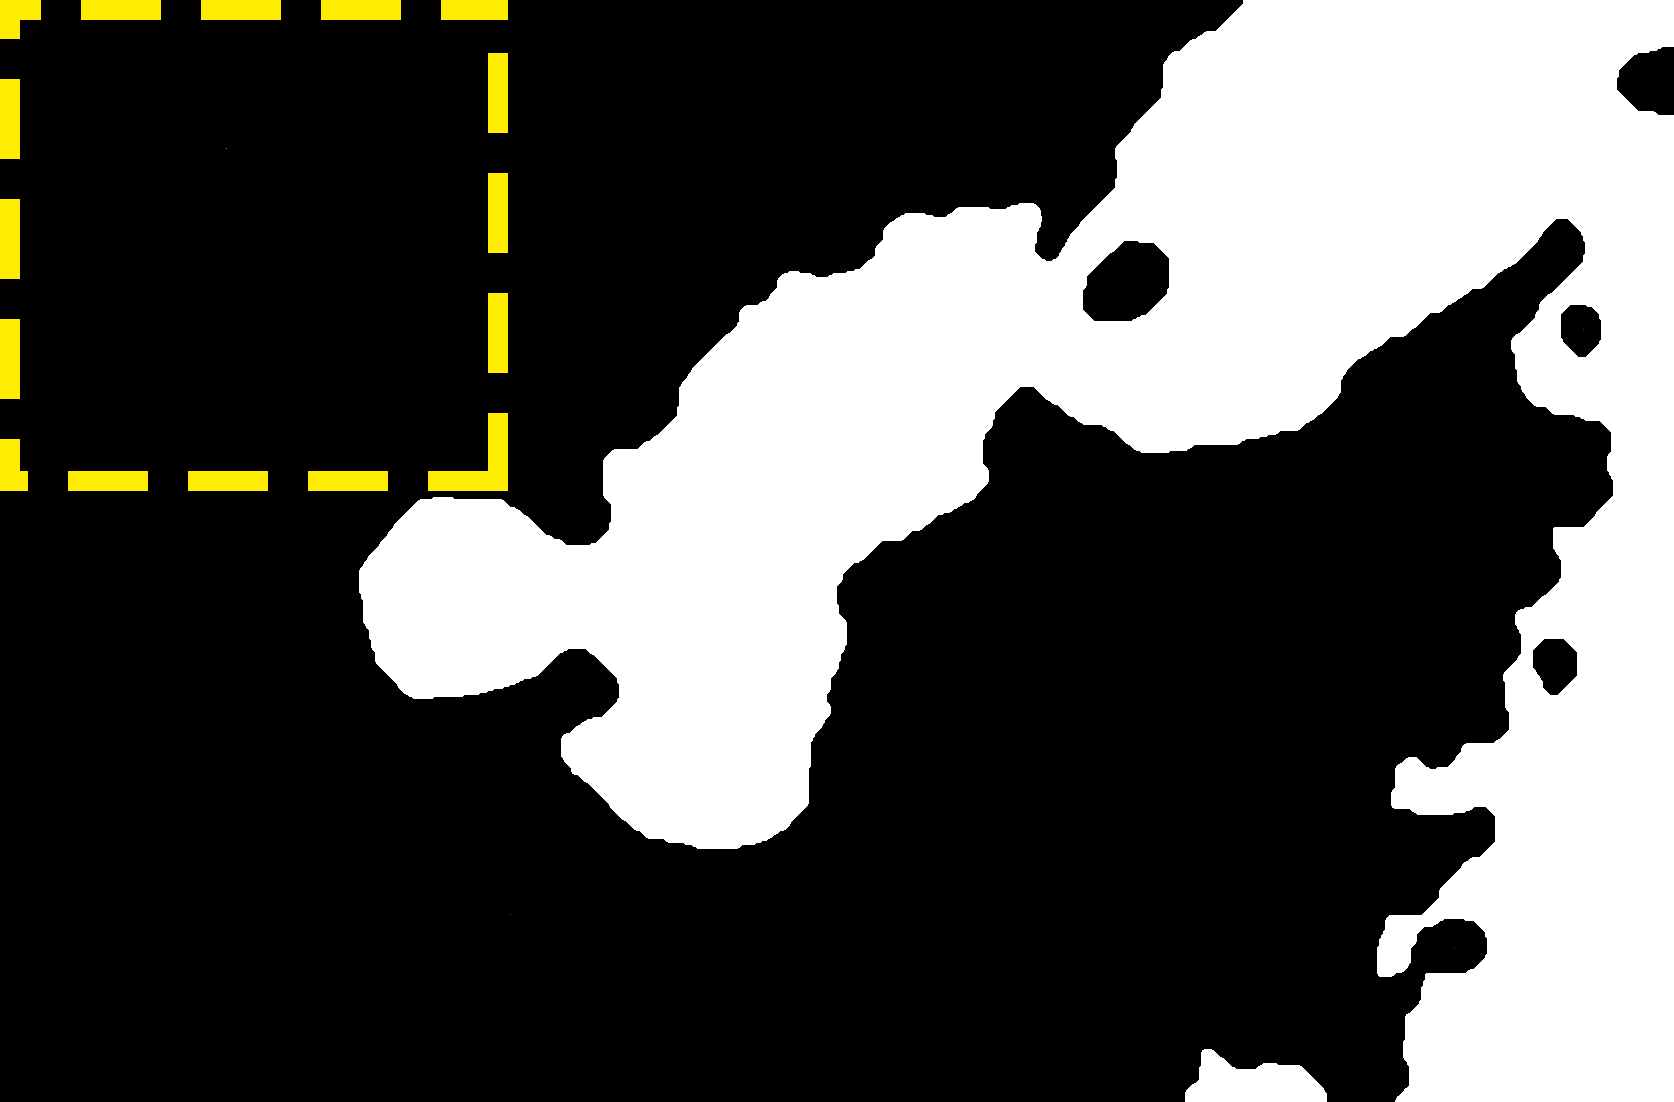
\includegraphics[width=0.8\linewidth]{Bilder/Aufgabe3/Einsparung_Fluege.png}
    \caption{Das einzelne Scannen dieses Bereiches würde ungefähr \textbf{63 tausend Flüge einsparen}.}
\end{figure}

Es lohnt sich also groß anzufangen und nicht direkt auf der niedrigsten Höhe die Map zu untersuchen.
\\[0.4cm]
Zusätzlich würde es nicht ausreichen das Gebiet in nebeneinander liegende 20x20 Quadrate zu unterteilen, da es so zu einem Sonderfall kommen könnte.
\\[0.4cm] 
In der Aufgabenstellung ist definiert, dass Quax zwar ein 20x20 gemischtes Quadrat überqueren kann, jedoch kein 20x20 Wasser-Quadrat.

Nun kann es dazu kommen, dass zwei benachbarte, gemischte 20x20 Quadrate ein quasi „unentdecktes“ 20x20 Wasser-Quadrat zwischen sich haben (siehe Abbildung 27). In diesem Fall würde ein normaler Wegfindungs-Algorithmus Quax diese zwei 20x20 gemischten Quadrate überqueren lassen. Jedoch müsste Quax dafür auch ein 20x20 Wasser-Quadrat überqueren, was nicht geht.
\begin{figure}[H]
\centering
    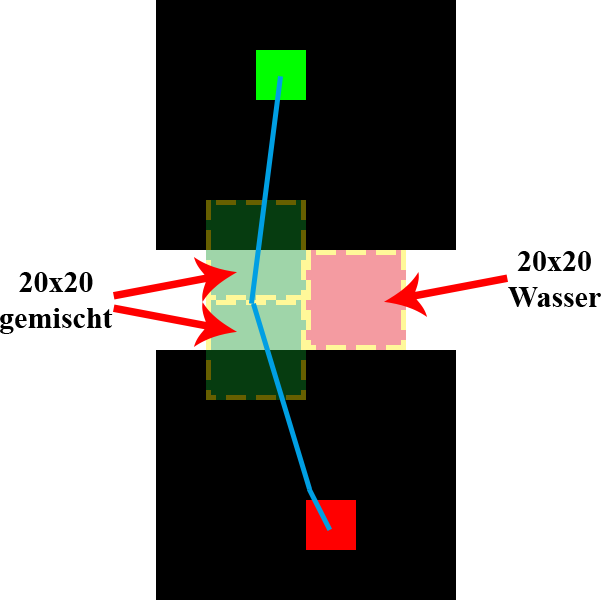
\includegraphics[width=0.8\linewidth]{Bilder/Aufgabe3/Sonderfall.png}
    \caption{Bei einer Überquerung der beiden Linken 20x20 Quadrate, würde Quax das eigentliche 20x20 Wasser-Quadrat einfach „überspringen“.}
\end{figure}

\subsection{Lösungsidee}
% TODO: QUELLE: QUADTREE
Um die Map mit möglichst wenig Flügen zu untersuchen, eignet es sich einen Quadtree („Quaternärbaum“) zu verwenden. Ein Quadtree ist eine Baum-Datenstruktur, bei der jeder innere Knoten genau vier Tochterknoten hat. Quadtrees werden in der Informatik oft zur Unterteilung von Bildern verwendet.
\\[0.4cm]
Diese Datenstruktur eignet sich hervorragend für die Unterteilung der Karte. Ein größeres Quadrat würd dabei in jeweils 4 gleichgroße kleinere Quadrate unterteilt (siehe Abbildung 28).
\begin{figure}[H]
\centering
    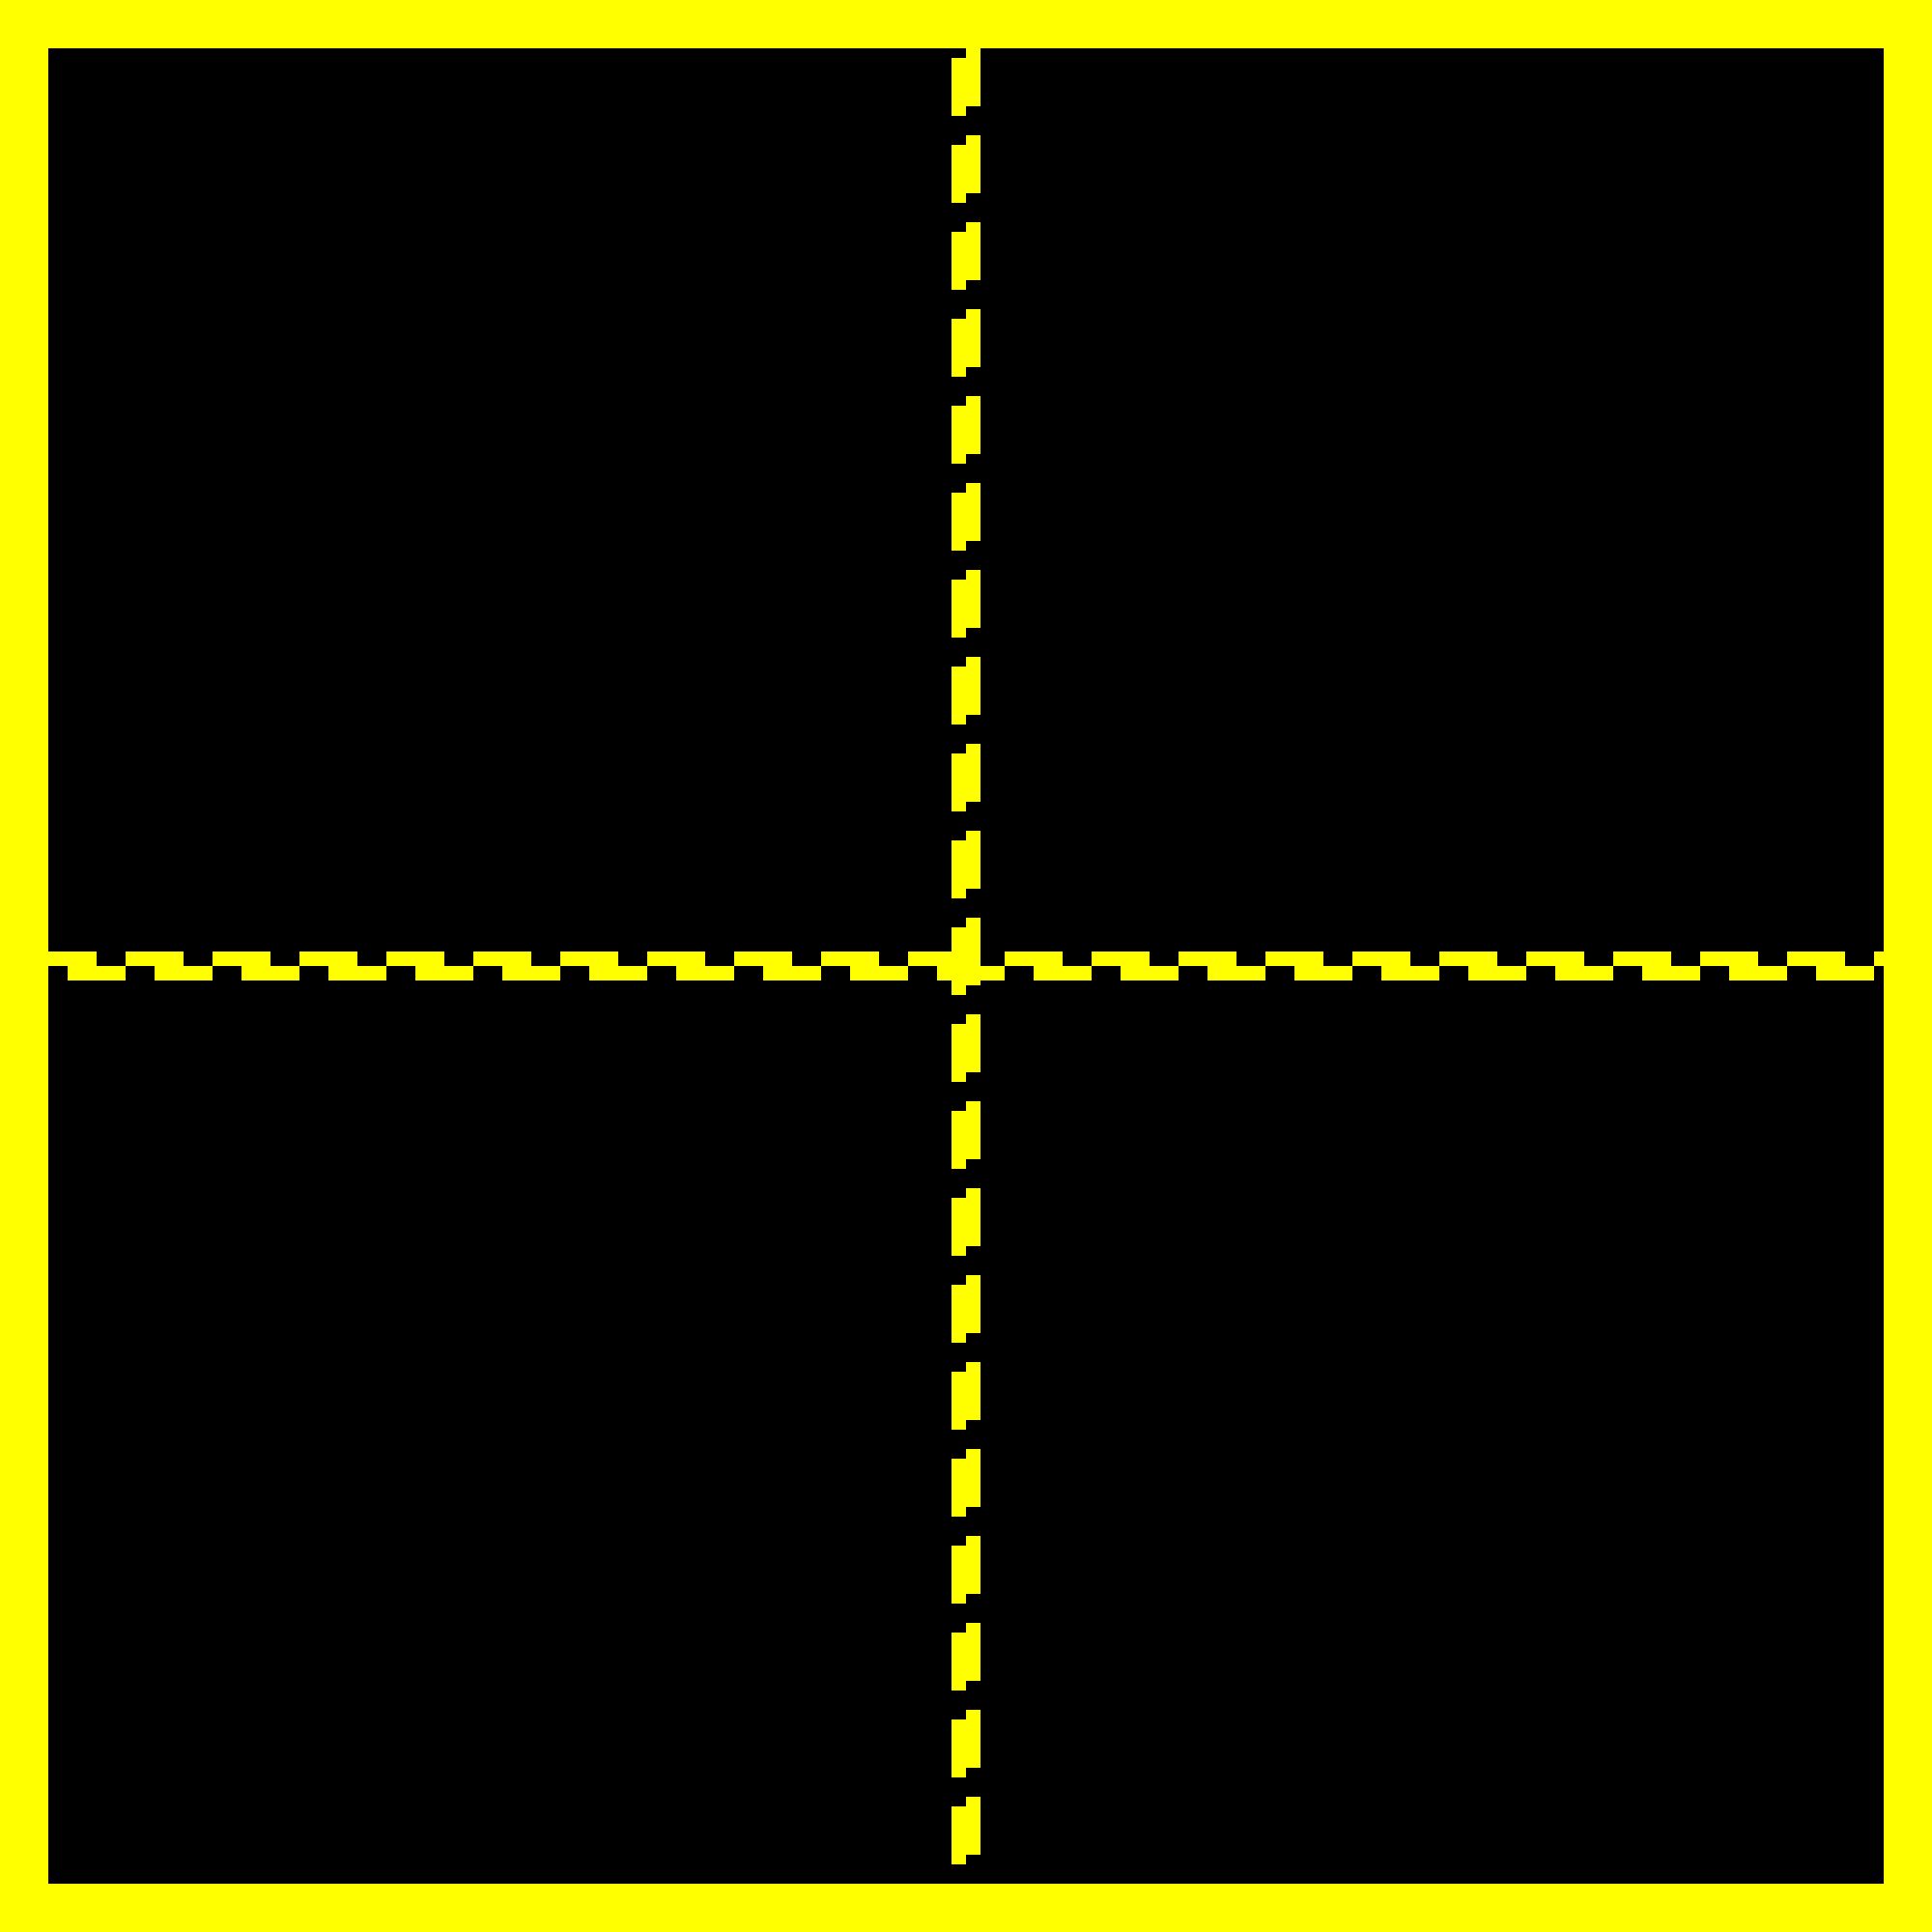
\includegraphics[width=0.5\linewidth]{Bilder/Aufgabe3/Quadtree_Einfach.png}
    \caption{Das größere Quadrat wird in jeweils 4 gleichgroße, kleinere Quadrate unterteilt. Das große Quadrat Objekt, hält dabei eine Referenz auf die Kleineren.}
\end{figure}

Man teilt ein Quadrat immer dann auf, wenn der jeweilige Inhalt nicht eindeutig als Land oder Wasser bestimmt werden kann, und das Quadrat noch größer als 20x20 ist.

Abbildung 29 zeigt eine solche Unterteilung für eine Beispielkarte. Es wird nach Quaxs Position (1, 10) gesucht. Hierbei wird zuerst die Wurzel des Quadtrees gebildet, welche die gesamte Karte beinhaltet. Nachdem diese als gemischt identifiziert wird (1. Flug), wird die Wurzel unterteilt. Da das Süd-Westliche Quadrat den Punkt (1, 10) enthält, wird dieses als nächstes angeflogen (2. Flug). Da jedoch auch dieses das Ergebnis „Gemischt“ zurückliefert, wird es auch unterteilt. Das Süd-Westliche innere Quadrat ist wieder das, welches die Position (1, 10) enthält und wird somit untersucht (3. Flug). Da dieses jedoch eindeutig Land enthält, ist die Unterteilung abgeschlossen.
\begin{figure}[H]
\centering
    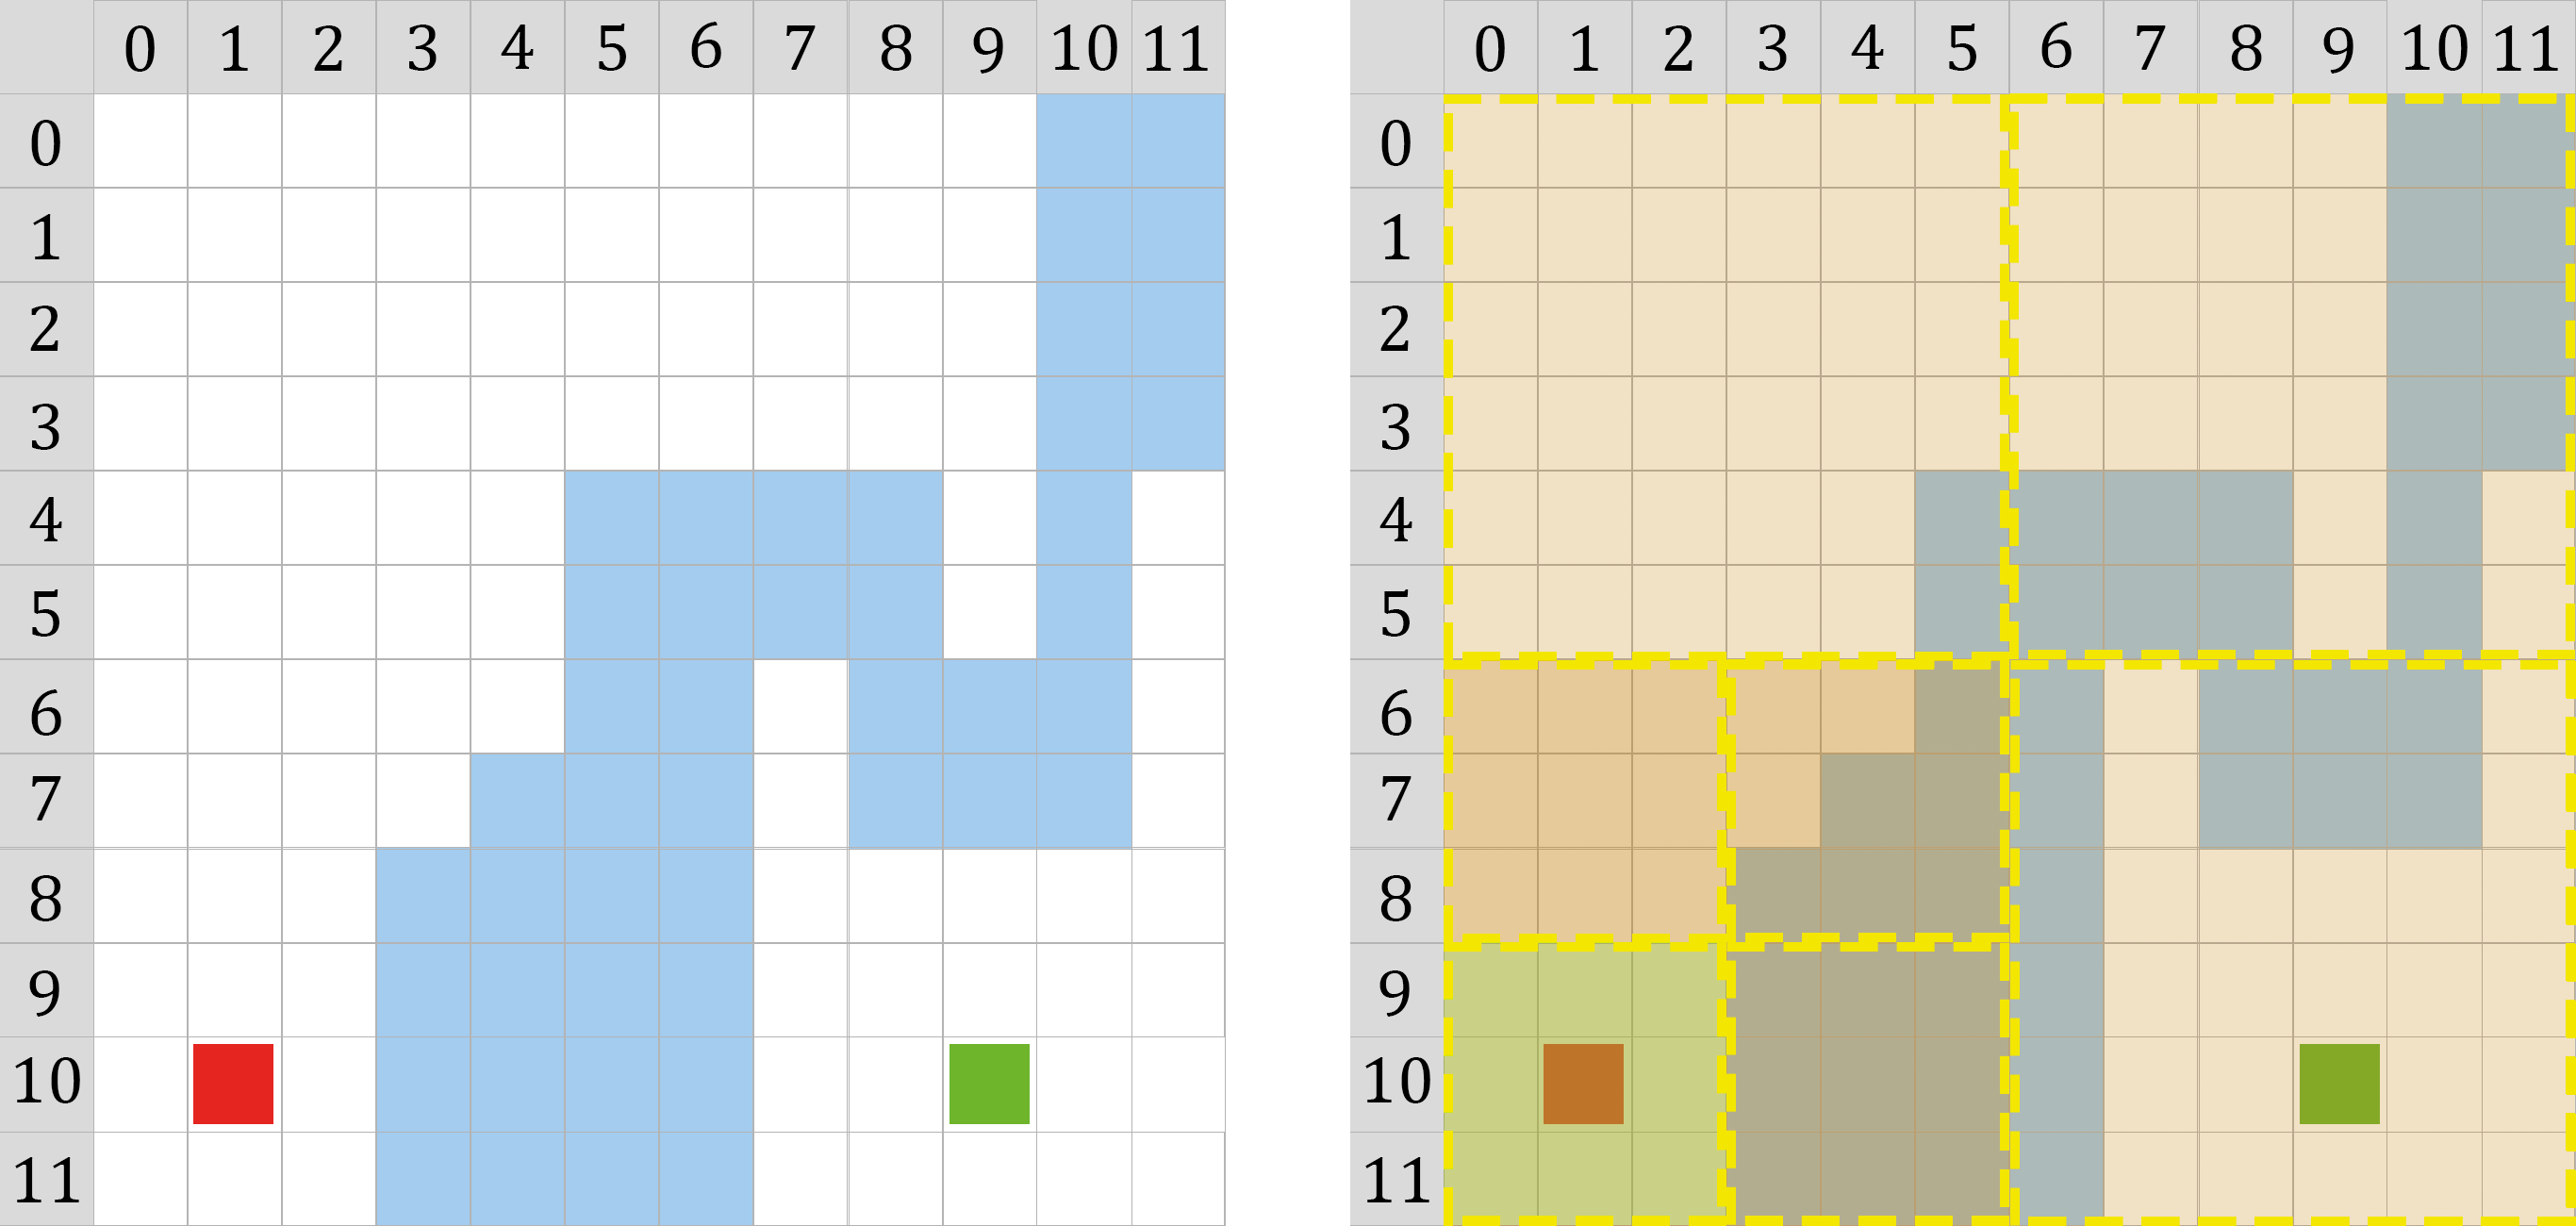
\includegraphics[width=1\linewidth]{Bilder/Aufgabe3/Quadtree_01.png}
    \caption{Für die links abgebildete Karte wird ein Quadtree (rechts) so gebildet, dass Quaxs Umgebung eindeutig bestimmt werden kann.}
\end{figure}

Nun stellt diese Quadtree Struktur aber auch eine Bedingung an die zu untersuchende Karte. Da der Quadcopter immer Viereckige Gebiete untersucht und die Wurzel des Quadtree-Baums die gesamte Karte umfassen muss, muss die Karte auch quadratisch sein. Dies ist jedoch kein größeres Problem, da in der Aufgabenstellung festgelegt wurde, dass alle Bereiche außerhalb der definierten Karte als Wasser angenommen werden können.
\\[0.4cm]
Jetzt gibt es aber auch beim Quadtree den Sonderfall, dass ein Quadrat mit ungerader Größe unterteilt werden muss. Dabei, wenn man alle Bereiche abdecken will, kommt es zu Überlappungen der inneren Quadrate (siehe Abbildung 29).
\begin{figure}[H]
\centering
    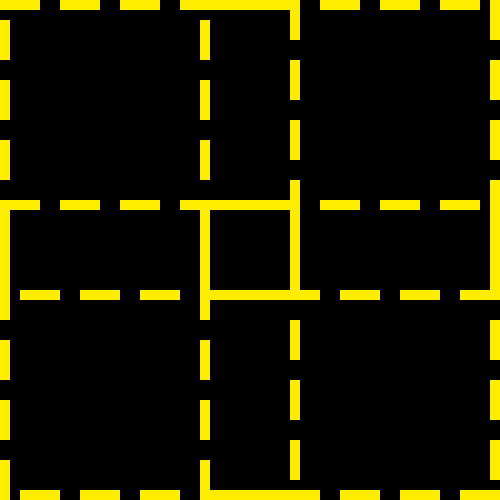
\includegraphics[width=.5\linewidth]{Bilder/Aufgabe3/Quadtree_Ueberlappung.png}
    \caption{Bei einer Aufteilung eines Quadrats mit ungerader Größe überlappen sich die inneren Quadrate.}
\end{figure}

Um dies zu verhindern könnte man die Karte nicht einfach nur quadratisch machen, sondern auf eine Größe bringen, so dass die Breite und Höhe der Map einer Zweierpotenz entsprechen. Dadurch könnte jede Aufteilung bis zum kleinst-möglichen 20x20 Quadrat ohne Überlappungen durchgeführt werden.
\\[0.4cm]
Der Nachteil dieser Skalierung ist jedoch eine ziemliche Vergrößerung der Karte im Vergleich zur ersten Methode (siehe Abbildung 31).
\begin{figure}[H]
\centering
    
\includegraphics[width=.9\linewidth]{Bilder/Aufgabe3/Erweiterung_Karte.png}
    \caption{Links die einfache Umformung der Map zu einem Quadrat so dass Breite = Höhe. Rechts die Umformung zu einer Zweierpotenz-Größe. Der blau markierte Bereich zeigt jeweils die zusätzlich hinzugefügten Gebiete an.}
\end{figure}

Für noch größere Karten steigt der Unterschied zwischen den beiden Methoden noch mehr und je größer die Karte, desto mehr Quadcopter Flüge bis man das eigentliche Gebiet erreicht hat.
\\[0.4cm]
Um nun auch auf den Sonderfall der zwei angrenzenden, gemischten 20x20 Quadrate, zwischen denen ein 20x20 Wasser Quadrat liegt, Rücksicht zu nehmen, darf der Weg zur Stadt nicht aus 20x20 aneinanderliegenden Quadraten bestehen, sondern aus 20x20 überlappenden Quadraten.

Auf diese Weise kann sichergestellt werden, dass keine 20x20 Wasser-Quadrate, die zwischen zwei 20x20 gemischten Quadraten liegen übersprungen werden.

\subsection{Teilaufgabe (a)}
Ein Quadrat in der Landschaft kann für Quax drei mögliche Zustände Wasser („W“), Land („L“) oder Unbekannt („U“) haben.

% TODO: A* und Dijkstra quelle
Als Wegfindungs-Algorithmus wird \textbf{A* (A-Star)} verwendet. A* ist eine Variante des Dijkstra-Algorithmus, die auf einem vorher schon angesprochenem Grid-System beruht (siehe Abbildung 32). Die einzelnen Elemente des Grids werden als „Nodes“ bezeichnet.
\begin{figure}[H]
\centering
    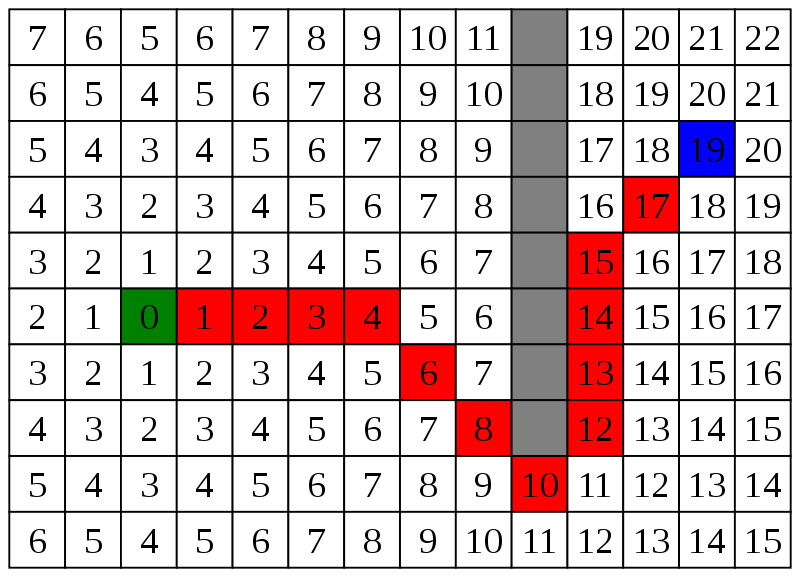
\includegraphics[width=.8\linewidth]{Bilder/Aufgabe3/Teilaufgabe_A/AStar_01.png}
    \caption{Findung des kürzesten Wegs vom grünen zum blauen Quadrat durch A*. Hierbei ist nur der Weg markiert und nicht alle untersuchten Nodes. Die Zahlen geben die Entfernung in Nodes zum Ausgangspunkt an.}
\end{figure}

Die generelle Funktionsweise des A* Algorithmus soll hier nur kurz erklärt werden. Für eine umfassendere Erklärung werden die zu diesem Thema im Literaturverzeichnis angegebenen Quellen empfohlen.
\\[0.4cm]
Der A* Algorithmus beginnt mit einer Start-Node (\code{S}), einer Target-Node (\code{T}), einem \code{openSet} und einem \code{closedSet}. Jede Node hat dabei entweder den Status „Walkable“ oder „Unwalkable“. Es werden zuerst alle Nachbar-Nodes von \code{S} mit dem Zustand „Walkable“ zum \code{openSet} hinzugefügt. Für sie werden jeweils 3 Werte berechnet. \code{G-Cost} beschreibt die Entfernung zu \code{S}. \code{H-Cost} beschreibt die Entfernung zu \code{T}. \code{F-Cost} entspricht \code{G-Cost} + \code{H-Cost}. (Für die Berechnung dieser \code{F-Cost} gibt es mehrere Varianten. Hier wird die sogenannte „Manhatten-Distanz“ verwendet.)
\\[0.4cm]
Als nächstes wird die Node im \code{openSet} mit der geringsten \code{F-Cost} aus dem \code{openSet} entfernt und dem \code{closedSet} hinzugefügt. Für diese Node werden wieder alle Nachbarn mit dem Status „Walkable“ entweder in das \code{openSet} aufgenommen und ihre Werte berechnet oder, falls sie schon im \code{openSet} vorhanden sind, werden ihre Werte aktualisiert.
\\[0.4cm]
Dieser Vorgang wiederholt sich so lange, bis \code{T} erreicht wurde.
\\[0.4cm]
Das hier auftretende Problem ist, dass bei einem normalen A* Algorithmus vorher schon das gesamte Grid definiert sein muss. Der Algorithmus muss wissen, welche Nodes „Walkable“ und welche „Unwalkable“ sind um einen Pfad zu finden.

Da das Scannen der gesamten Map jedoch auch mit der Quadtree Struktur viel zu viele letztendlich Quadcopter Flüge beanspruchen würde, gibt es bei der hier verwendeten A* Variante noch den dritten möglichen Node Status „Unknown“.

Wie genau der Algorithmus mit einem dritten Status abläuft, wird nun an einem kleinen Beispiel veranschaulicht.
\\[0.4cm]
Zu Beginn hat jede Grid-Node außer \code{S} und \code{T}, die beide den Status „Walkable“ haben, den Status „Unknown“ (siehe Abbildung 33). 
\begin{figure}[H]
\centering
    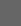
\includegraphics[width=.5\linewidth]{Bilder/Aufgabe3/Teilaufgabe_A/Beispiel_01.png}
    \caption{Die Map aus A* Sicht. Alle Nodes des Status „Unknown“ sind grau markiert.}
\end{figure}
Nun wird der erste Flug durchgeführt und die Grid-Nodes dementsprechend aktualisiert (siehe Abbildung 34).
\begin{figure}[H]
\centering
    
\includegraphics[width=.5\linewidth]{Bilder/Aufgabe3/Teilaufgabe_A/Beispiel_02.png}
    \caption{Durch den ersten Flug wurde der Status von einigen Nodes um Quax aufgedeckt. Schwarz steht für „Walkable“, Weiß für „Unwalkable“.}
\end{figure}
Danach wird zuerst der A* Pathfinding Algorithmus normal durchgeführt. Das heißt, dass nur Nodes mit dem Status „Walkable“ auch als tatsächlich begehbar angenommen werden. Die restlichen Nodes mit dem Status „Unknown“ oder „Unwalkable“ gelten als nicht begehbar.
\\[0.4cm]
Wird so ein Weg zum Ziel gefunden ist der Algorithmus fertig und es steht fest, dass es einen Pfad zur Stadt gibt. Umgekehrt heißt jedoch nicht, dass wenn kein Weg gefunden wurde es keinen Weg gibt. Stattdessen führt man eine zweite A* Suche durch bei der diesmal nicht nur Nodes des Status „Walkable“, sondern auch die des Status „Unknown“ als begehbar betrachtet werden.
\\[0.4cm]
Findet diese Suche wiederum einen Pfad zum Ziel, bedeutet das, dass noch weitere Flüge zur Erkundung dieser „Unknown“-Nodes notwendig sind, um sagen zu können, ob es einen Pfad gibt oder nicht.
Findet dagegen auch die zweite Suche keinen Weg zur Stadt, so bedeutet das, dass es auch wirklich keinen Weg gibt.
\\[0.4cm]
Abbildung 35 zeigt die notwendige Durchführung weiterer Flüge zur Findung eines Pfades.
\begin{figure}[H]
\centering
    
\includegraphics[width=1\linewidth]{Bilder/Aufgabe3/Teilaufgabe_A/Beispiel_03.png}
    \caption{Da auch nach einem weiteren Flug (links) noch nicht offensichtlich ist, ob es einen Weg gibt oder nicht, wird ein dritter (rechts) durchgeführt.}
\end{figure}
Bei der Durchführung des ersten A* Algorithmus wird nun ein Weg aus nur „Walkable“-Nodes gefunden. Damit ist das Pathfinding abgeschlossen. Es wurde ein Weg gefunden (siehe Abbildung 36).
\begin{figure}[H]
\centering
    
\includegraphics[width=.5\linewidth]{Bilder/Aufgabe3/Teilaufgabe_A/Beispiel_04.png}
    \caption{Die Vollständige Map. Der Pfad zur Stadt ist pink eingezeichnet.}
\end{figure}

\subsection{Teilaufgabe (b)}
Der Schlüssel zu einem möglichst effizienten Algorithmus, welcher nur wenige Quadcopter-Flüge benötigt, ist die Koordinierung zwischen dem A* Pathfinding und der Quadtree Datenstruktur.
\\[0.4cm]
Das A* Grid wird nur mit den nötigsten „Informationen versorgt“.
Der Quadtree muss vorbereitet sein vom A* Pathfinding aus eine Anforderung für das Scannen eines Bereiches zu bekommen. Dieser Bereich muss dann identifiziert werden und zurück an das Pathfinding System gegeben werden, welches mit dem Resultat das eigene A* Grid aktualisiert und die Wegsuche neu startet.
\\[0.4cm]
Ein weiterer nicht zu vernachlässigender Aspekt ist das Umgehen mit dem Sonderfall, dass Quax über ein 20x20 Wasser-Quadrat drüber kommt durch zwei aneinanderliegende, gemischte 20x20 Quadrate.
Um dies zu verhindern ist 
Das A* Grid wird zwar aus 10x10 breiten Nodes bestehen, jedoch wird auf den Sonderfall dadurch geachtet, dass der Status jeder einzelnen Grid-Node jeweils dem Map-Status des 20x20 Map-Quadrats entspricht, dessen linke, untere Ecke die gleichen Koordinaten hat wie die Grid-Node (siehe Abbildung 33).

\begin{figure}[H]
\centering
    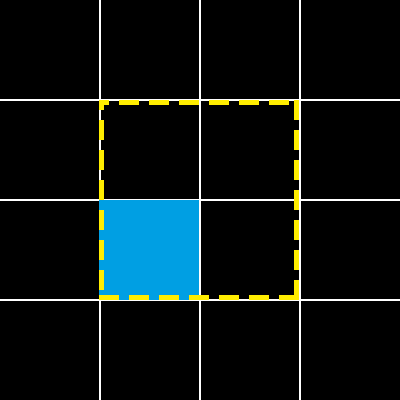
\includegraphics[width=.8\linewidth]{Bilder/Aufgabe3/Teilaufgabe_A/AStar_Grid.png}
    \caption{Der blaue Pixel repräsentiert eine Node im A*-Grid. Der Status dieser Node wird jedoch über den Map-Typ des gelben Quadrats definiert. Beinhaltet dieses zum Beispiel nur Land, ist die Grid-Node „Walkable“.}
\end{figure}

Dadurch entsteht letztendlich ein Geflecht aus überlappenden 20x20 Quadraten, welches wiederum den Sonderfall abdeckt (siehe Abbildung 34).

\begin{figure}[H]
\centering
    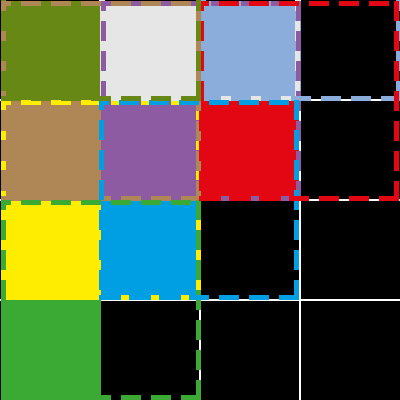
\includegraphics[width=.8\linewidth]{Bilder/Aufgabe3/Teilaufgabe_A/AStar_Grid_02.png}
    \caption{Ein Geflecht aus Grid-Nodes und den jeweils dazugehörigen Map-Quadraten. Die 2x2 Map-Quadrate überlappen sich sichern somit den Sonderfall ab.}
\end{figure}

\subsection{Teilaufgabe (c)}
\subsubsection{Implementierung}
% WIESO UNITY
% MULTITHREADING UND EVENTS
% A*
% QUADTREE
\subsubsection{Optimierungsmöglichkeiten}
Die Algorithmuslaufzeit der aktuelle Implementierung ist gerade für größere Maps sehr schlecht. Dabei überrascht, dass die einzelnen Komponente eigentlich gar nicht viel Zeit verbrauchen. Das Suchen im Quadtree, das Aktualisieren des A* Grids und die erste Wegsuche verbrauchen alle zusammen nur wenige Millisekunden pro Durchgang. 
\\[0.4cm]
Das was am meisten Zeit verbraucht ist die zweite Wegsuche. Nicht zuletzt, weil sie noch nicht durch Caching optimiert ist. Allerdings erklärt auch die Laufzeit des zweiten Pathfinding-Algorithmus nicht die Länge der Gesamtlaufzeit. Die Wahl einer Game-Engine als Entwicklungsumgebung hat die Performance letztendlich durch Hintergrundprozesse doch eher um einiges verschlechtert als verbessert.
\\[0.4cm]
Mögliche Optimierungsmöglichkeiten zur Verbesserung der Laufzeit oder Verringerung der benötigten Quadcopter Flüge wären:
\\[0.4cm]
\textbf{Multithreading}

Nicht alle Bestandteile des Algorithmus nutzen das Prinzip des Multithreadings optimal aus und können noch erheblich verbessert werden.
\\[0.4cm]
\textbf{A* Pathfinding}

A* ist ein Pathfinding-Algorithmus zum Finden eines kürzesten oder zumindest möglichst kurzen Weges. Jedoch ist für diese Aufgabenstellung die Länge des Weges irrelevant und viele der Quadcopter Flüge zum Erkunden sehr kleiner Gebiete sind nicht unbedingt notwendig. Um dieses Verhalten des A*-Algorithmus zumindest abzuschwächen, könnte man noch weitere Heuristiken implementieren.
\\[0.4cm]
\textbf{Speichern von Pathfinding Zuständen}

Das bereits implementierte Caching für eine Wegfindung, bei der noch unbekannte Nodes als nicht-betretbar angenommen werden, hat die Laufzeit erheblich minimiert.

Nun ist es aber noch möglich Zustände für die Wegfindung, bei der unbekannte Nodes als betretbar angenommen werden, zu speichern, so dass dieser Algorithmus nicht jedes mal von der Startposition bis zur Zielposition suchen muss, sondern auf vorher durchgeführte Suchergebnisse zurückgreifen kann.
\\[0.4cm]
\textbf{Verbindung beider A* Suchen}

Eine Alternative zum Speichern des aktuellen Zustandes der zweiten A* Suche, wäre auch eine Integration dieser in die schon vorherige A* Suche. Indem man alle unbekannten Nachbar-Nodes in einem zweiten \code{openSet} speichert und nach fehlgeschlagener ersten Suche eine Zweite mit dem zusätzlich erstellten \code{openSet} und der Bedingung, unbekannte Nodes begehbar sind, lässt einiges an Laufzeit einsparen.
\\[0.4cm]
\textbf{Bidirektionale Suche}

% TODO: QUELLE BIDIREKTIONALE SUCHE
Mit Hilfe einer „Bidirektionale Suche“, könnte sich sowohl die Laufzeit, als auch die benötigte Anzahl an Quadcopter Flügen weiter verbessern.
\\[0.4cm]
\textbf{Unity Implementierung}

Die Wahl einer Game-Engine als Entwicklungsumgebung hat auch einen sehr großen Einfluss auf die Laufzeit, durch viele für dieses Programm unnötige Hintergrundprozesse. Auch das einzelne Darstellen von Flügen auf der Map-Textur verbraucht viele Ressourcen. Die Laufzeit des puren Algorithmus ist daher wesentlich geringer als die Zeit, die das Programm für die fertige Abbildung des Weges benötigt.

Eine simplere Konsolen-Anwendung, die dem Benutzer die Flüge am Ende in eine PNG-Datei einträgt, würde zum Beispiel nochmals deutlich effizienter laufen.


\subsubsection{Beispiele}
% TODO: BEISPIELE

\subsection{Teilaufgabe (d)}
Mit einer eher unnatürlichen Verteilung von Flüssen und Seen wie zum Beispiel einem Schachbrettmuster (siehe Abbildung ||||), einem verzweigten Labyrinth (siehe Abbildung ||||) oder eine Anordnung mehrerer schmaler Wasser und Land streifen (siehe Abbildung ||||), können kaum noch größere Flächen eindeutig eingeteilt werden.

Dies sorgt schnell für einen sehr umfangreichen Quadtree und damit auch für viele Quadcopter Flüge.
\\[0.4cm]
Der hier besprochene Algorithmus läuft am effizientesten, bei eher natürlichen Landschaften, mit größeren Wasser- und Landflächen. Dabei kann der Quadcopter den Typ größere Gebiete mit nur einem Flug identifizieren.

\begin{figure}[H]
\centering
    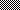
\includegraphics[width=0.7\linewidth]{Bilder/Aufgabe3/Teilaufgabe_D/schachbrett.png}
    \caption{Schachbrettartige Landverteilung}
\end{figure}
\begin{figure}[H]
\centering
    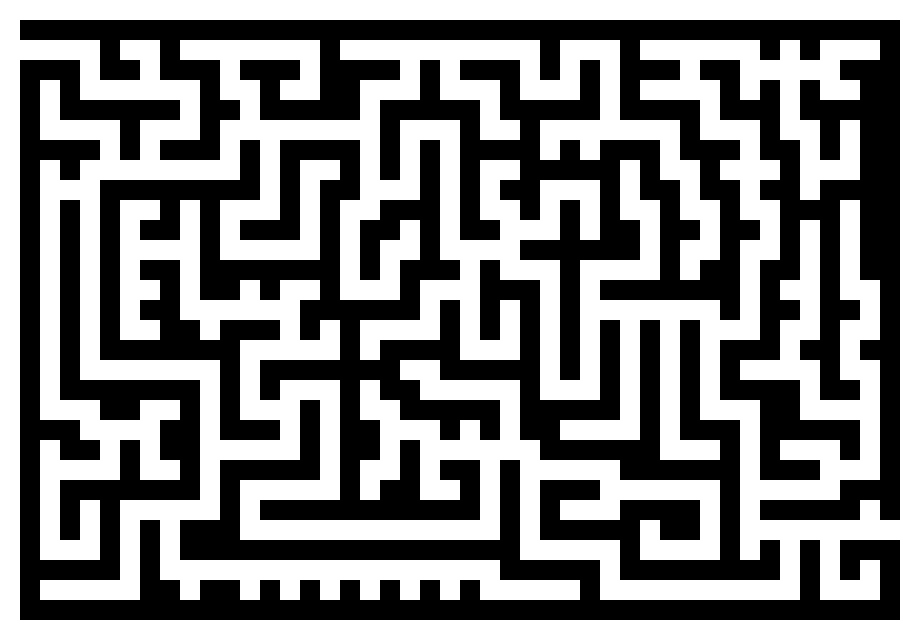
\includegraphics[width=0.7\linewidth]{Bilder/Aufgabe3/Teilaufgabe_D/irrgarten.png}
    \caption{Irrgarten ähnliche Landverteilung}
\end{figure}
\begin{figure}[H]
\centering
    
\includegraphics[width=0.7\linewidth]{Bilder/Aufgabe3/Teilaufgabe_D/linien.png}
    \caption{Linienartige Landverteilung}
\end{figure}


%===================================================================================
%---------------------------------- FAZIT ------------------------------------------
%===================================================================================

\newpage
\section{FAZIT}
Lorem ipsum dolor sit amet, consectetur adipiscing elit. Sed tempus consectetur lorem, imperdiet dignissim est auctor a. Vivamus convallis, leo et iaculis egestas, nunc massa porttitor tellus, id faucibus urna justo eget massa. Praesent quis feugiat odio. Nullam quis mattis enim. Fusce volutpat odio in enim sodales venenatis. Mauris consequat.


%===================================================================================
%--------------------------- LITERATURVERZEICHNIS ----------------------------------
%===================================================================================

\newpage
\section{LITERATURVERZEICHNIS}

\begingroup
\renewcommand{\section}[2]{}%
\begin{large}
\textbf{Buchquellen:}
\end{large}

\begin{thebibliography}{9}

    \bibitem{lamport94}
      Leslie Lamport,
      \textit{\LaTeX: a document preparation system},
      Addison Wesley, Massachusetts,
      2nd edition,
      1994.
      \bibitem{lamport91}
      Leslie Lamport,
      \textit{\LaTeX: a document preparation system},
      Addison Wesley, Massachusetts,
      2nd edition,
      1994.
      \bibitem{lamport97}
      Leslie Lamport,
      \textit{\LaTeX: a document preparation system},
      Addison Wesley, Massachusetts,
      2nd edition,
      1994.

\end{thebibliography}

\vspace{1cm}

\begin{large}
\textbf{PDF-Scans:}
\end{large}

\begin{thebibliography}{9}

    \bibitem{bwinf_runde1_ergebnis}
      Leslie Lamport,
      \textit{\LaTeX: a document preparation system},
      Addison Wesley, Massachusetts,
      2nd edition,
      1994.
  	\bibitem{bwinf_runde2_ergebnis}
      Leslie Lamport,
      \textit{\LaTeX: a document preparation system},
      Addison Wesley, Massachusetts,
      2nd edition,
      1994.

\end{thebibliography}

\vspace{1cm}

\begin{large}
\textbf{Internetquellen:}
\end{large}

\begin{thebibliography}{9}

    \bibitem{lamport94}
      Leslie Lamport,
      \textit{\LaTeX: a document preparation system},
      Addison Wesley, Massachusetts,
      2nd edition,
      1994.
      \bibitem{lamport91}
      Leslie Lamport,
      \textit{\LaTeX: a document preparation system},
      Addison Wesley, Massachusetts,
      2nd edition,
      1994.
      \bibitem{lamport97}
      Leslie Lamport,
      \textit{\LaTeX: a document preparation system},
      Addison Wesley, Massachusetts,
      2nd edition,
      1994.

\end{thebibliography}

\endgroup

%===================================================================================
%--------------------------- ABBILDUNGSVERZEICHNIS ---------------------------------
%===================================================================================

\newpage
\section{ABBILDUNGSVERZEICHNIS}
Die meisten enthaltenen Abbildungen wurden entweder selbst mit unten aufgelisteten Tools erstellt oder von unten genannten Programmen/Quellen aufgenommen.
\begin{itemize}
\item Microsoft PowerPoint
\item Adobe Photoshop CC 2018
\item UMLet
\item Grafikrechner - GeoGebra
% TODO: QUELLEN REFERENZIEREN 
\item BwInf36 Runde 2 Aufgabenstellung
\item Windows 10 Konsole
\end{itemize}

Sonstige Bildquellen:
\begin{itemize}
\item https://upload.wikimedia.org/wikipedia/commons/d/df/ZweiWegeIrrgarten.png
\item https://de.wikipedia.org/wiki/Datei:Pathfinding\_A\_Star.svg
\end{itemize}

%===================================================================================
%--------------------------- CD-VERZEICHNIS ----------------------------------
%===================================================================================

\newpage
\section{CD-VERZEICHNIS}

\begin{figure}[H]
    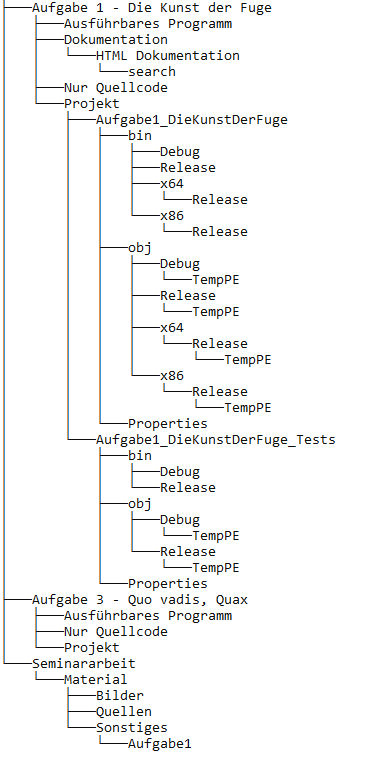
\includegraphics[width=.7\linewidth]{Bilder/Sonstiges/CDVerzeichnis.png}
\end{figure}

%===================================================================================
%--------------------------- ANHANG ----------------------------------
%===================================================================================

\newpage
\section{ANHANG}
Aufgrund der Länge des Quellcodes beider Aufgaben, werden die einzelnen Klassen hier nicht weiter aufgelistet.

Die einzelnen Quellcode-Dateien befinden sich auf der beigelegten CD.

\subsection{Installationshinweise}
Die Programme beider Aufgaben wurden kompiliert und befinden sich als ausführbare .exe Dateien auf der beigelegten CD.

Für beide Aufgaben wurden jeweils für Windows 64bit und 86bit Dateien erstellt.

%===================================================================================
%------------------------- ERKLÄRUNG DES VERFASSERS --------------------------------
%===================================================================================

\newpage
\section{ERKLÄRUNG DES VERFASSERS}

\begin{figure}[H]
    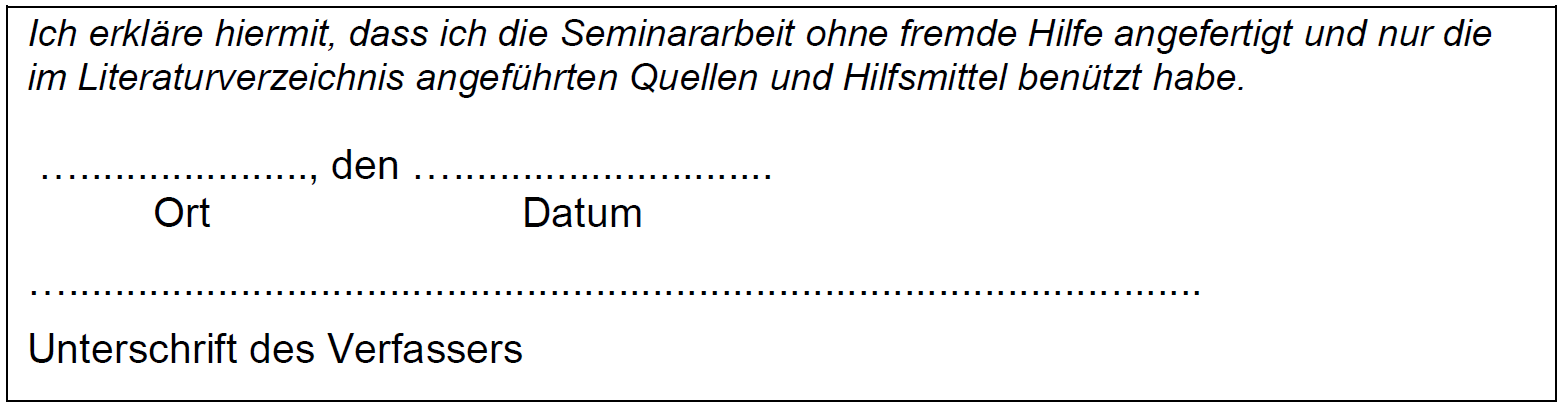
\includegraphics[width=\linewidth]{Bilder/Sonstiges/ErklaerungDesVerfassers.png}
\end{figure}

\end{document}
